%\documentclass[sigchi, review]{acmart}
\documentclass{sigchi}


%%%%%%%%%%%%%%%%%%%%%%%%%%%%%%%%%%%%%%%%%%%%%%%%%%%%%%%%%%%%%%%%%%%%
% This is the only line you need to add to load the CHIZen packages
%%%%%%%%%%%%%%%%%%%%%%%%%%%%%%%%%%%%%%%%%%%%%%%%%%%%%%%%%%%%%%%%%%%%
%
%  This file imports each of the separate .tex files in this directory -- feel free to enable/disable each separately as you'd like
%


%
%   A bunch of common includes for text formatting, features. 
%
%Robert's accented character fix
\usepackage[utf8]{inputenc}

% Enables use of Chinese characters
\usepackage{CJKutf8}

% MARKDOWN
%
% TODO: Explore how useful this is for general-purpose HCI papers
%       - Tables/Figures need to be a separate thing, but useful for everything else?
%
\usepackage[footnotes,definitionLists,hashEnumerators,smartEllipses,hybrid]{markdown}


% Jim added this -- useful highlighting function \hl{}
%\usepackage{soul,color}

% Mark likes to add these options to his papers .... worth considering
\frenchspacing
\raggedbottom

% Lennart's acronym package
\usepackage[nolist]{acronym}

\begin{acronym}
\acro{ANOVA}{Analysis of Variance}
\acro{HCI}{Human-Computer Interaction}
\end{acronym}


% Jim's quotation stuff
%\renewenvironment{quote}{%
%  \list{}{%
%    \leftmargin0.4cm   % this is the adjusting screw
%    \rightmargin\leftmargin
%  }
%  \item\relax
%}
%{\endlist}

% Jim added this -- useful highlighting function \hl{}
%\usepackage{soul,color}



% Study Variables
% ----------------------------

% scale up the sc font slightly
\usepackage{letltxmacro,lipsum,relsize}
\LetLtxMacro{\oldscshape}{\scshape}
\renewcommand{\scshape}[1]{\oldscshape\relscale{1.2}#1}

% an experiment factor/variable
\newcommand{\f}[1]{\mbox{{\textsc{#1}}}\xspace}
% usage: \f{block}, \f{width}, etc.
% NOTE: need \xspace package to fix spacing issues
%       \mbox prevents breaking

% a code when qualitative coding 
\newcommand{\cd}[1]{\textit{``{#1}''}\xspace}
% usage: \cd{errors}, \cd{work}


%
%   Figures -- formerly IDEA Plots -- Wraps most features from PGFPlots
%       * Handles common formatting, defines some common graph types
%       * See file for detailed documentation
%
%%%%%%%%%%%%%%%%%%%%%%%%%%%%%%%%%%%%%%%%%%%%%%%%%
%  HOW TO USE
%%%%%%%%%%%%%%%%%%%%%%%%%%%%%%%%%%%%%%%%%%%%%%%%%
%
% Include this line at the top of your TeX  File: 
%
% %%%%%%%%%%%%%%%%%%%%%%%%%%%%%%%%%%%%%%%%%%%%%%%%%
%  HOW TO USE
%%%%%%%%%%%%%%%%%%%%%%%%%%%%%%%%%%%%%%%%%%%%%%%%%
%
% Include this line at the top of your TeX  File: 
%
% \input{IDEA_Plots.tex}
%
%
% Then, add graphs to your paper using the following template: 
%
%\begin{tikzpicture}
%\begin{axis}[<GRAPH TYPE>,
%	% X Axis options (xmin, xmax, xtick={})
%	% Y Axis options (ymin, ymax, ytick={})
%       ]
%
%    % DATA GOES IN HERE
%
%\end{axis}
%\end{tikzpicture}
%
%
% OR, for multiple plots use this template:
%
%\begin{tikzpicture}
%\begin{groupplot}[
%   group style={
%       group size= <COL> by <ROW>,
%       x descriptions at=edge bottom,
%       y descriptions at=edge left,
%       vertical sep=0pt,
%       horizontal sep=0pt},
%  <GRAPH TYPE>, 
%	% X Axis options (xmin, xmax, xtick={})
%	% Y Axis options (ymin, ymax, ytick={})
%      ]
%
%    % DATA GOES IN HERE
%
%\end{groupplot}
%\end{tikzpicture}
%
%
%
% The following graph types are defined in this library:
%
% IDEA bar - A clustered bar graph, similar to Excel
% IDEA tufte panel - a bare-bones bar graph, suitable for stacked panel graphs in Tufte's style
% .. more that aren't listed here
%




%%%%%%%%%%%%%%%%%%%%%%%%%%%%%%%%%%%%%%%%%%%%%%%%%
%   Common Includes
%%%%%%%%%%%%%%%%%%%%%%%%%%%%%%%%%%%%%%%%%%%%%%%%%
\usepackage{pgfplots}
\usepackage{pgfplotstable}
\usepgfplotslibrary{dateplot}
\usepgfplotslibrary{groupplots}


%\usetikzlibrary{external}
%\tikzexternalize[prefix=tikz/] % Must be in main .tex file?

\usetikzlibrary{pgfplots.statistics}
\usetikzlibrary{matrix}

\usepackage{bbding}

\pgfplotsset{compat=newest}

%%%%%%%%%%%%%%%%%%%%%%%%%%%%%%%%%%%%%%%%%%%%%%%%%
%   Colour Definitions
%%%%%%%%%%%%%%%%%%%%%%%%%%%%%%%%%%%%%%%%%%%%%%%%%

\definecolor{RYB1}{RGB}{141, 211, 199}
\definecolor{RYB2}{RGB}{255, 255, 179}
\definecolor{RYB3}{RGB}{190, 186, 218}
\definecolor{RYB4}{RGB}{251, 128, 114}
\definecolor{RYB5}{RGB}{128, 177, 211}
\definecolor{RYB6}{RGB}{253, 180, 98}
\definecolor{RYB7}{RGB}{179, 222, 105}

\pgfplotscreateplotcyclelist{colorbrewer-RYB}{
{RYB1!50!black,fill=RYB1},
{RYB2!50!black,fill=RYB2},
{RYB3!50!black,fill=RYB3},
{RYB4!50!black,fill=RYB4},
{RYB5!50!black,fill=RYB5},
{RYB6!50!black,fill=RYB6},
{RYB7!50!black,fill=RYB7},
}

\pgfplotscreateplotcyclelist{colorbrewer-RYB-plain}{
{RYB1},
{RYB2},
{RYB3},
{RYB4},
{RYB5},
{RYB6},
{RYB7},
}

%%%%%%%%%%%%%%%%%%%%
% WATERLOO PALETTES - DIGITAL
%%%%%%%%%%%%%%%%%%%%

\definecolor{AHSLight}{RGB}{0, 154, 166}
\definecolor{AHSDark}{RGB}{0, 127, 138}

\definecolor{ArtsLight}{RGB}{233, 131, 0}
\definecolor{ArtsDark}{RGB}{172, 97, 0}

\definecolor{EngineeringLight}{RGB}{204, 170, 255}
\definecolor{EngineeringDark}{RGB}{87, 6, 140}

\definecolor{EnvironmentLight}{RGB}{182, 191, 0}
\definecolor{EnvironmentDark}{RGB}{116, 120, 0}

\definecolor{MathLight}{RGB}{255, 136, 221}
\definecolor{MathDark}{RGB}{224, 36, 154}
 
\definecolor{ScienceLight}{RGB}{119, 187, 225}
\definecolor{ScienceDark}{RGB}{0, 115, 207}


\definecolor{SchoolRedLight}{RGB}{247, 119, 119}
\definecolor{SchoolRedDark}{RGB}{150, 23, 46}



\pgfplotscreateplotcyclelist{waterloo-light}{
{AHSLight!50!black,fill=AHSLight},
{ArtsLight!50!black,fill=ArtsLight},
{EngineeringLight!50!black,fill=EngineeringLight},
{EnvironmentLight!50!black,fill=EnvironmentLight},
{MathLight!50!black,fill=MathLight},
{ScienceLight!50!black,fill=ScienceLight},
{SchoolRedLight!50!black,fill=SchoolRedLight},
}

\pgfplotscreateplotcyclelist{waterloo-dark}{
{AHSDark!50!black,fill=AHSDark},
{ArtsDark!50!black,fill=ArtsDark},
{EngineeringDark!50!black,fill=EngineeringDark},
{EnvironmentDark!50!black,fill=EnvironmentDark},
{MathDark!50!black,fill=MathDark},
{ScienceDark!50!black,fill=ScienceDark},
{SchoolRedDark!50!black,fill=SchoolRedDark},
}



%%%%%%%%%%%%%%%%%%%%
% WATERLOO  PALETTES - PRINT
%%%%%%%%%%%%%%%%%%%%

% FIX: CMYK is conflicting with other colour definitions in SIGCHI template

%\definecolor{AHSPrint}{CMYK}{100, 0, 30, 2}
%\definecolor{ArtsPrint}{CMYK}{0, 52, 100, 0}
%\definecolor{EngineeringPrint}{CMYK}{24, 0, 98, 8}
%\definecolor{EnvironmentPrint}{CMYK}{78, 94, 0, 0}
%\definecolor{MathPrint}{CMYK}{5, 90, 0, 0}
%\definecolor{SciencePrint}{CMYK}{90, 48, 0, 0}
%\definecolor{SchoolRedPrint}{CMYK}{3, 100, 66, 12}

%\pgfplotscreateplotcyclelist{waterloo-print}{
%{AHSPrint!50!black,fill=AHSPrint},
%{ArtsPrint!50!black,fill=ArtsPrint},
%{EngineeringPrint!50!black,fill=EngineeringPrint},
%{EnvironmentPrint!50!black,fill=EnvironmentPrint},
%{MathPrint!50!black,fill=MathPrint},
%{SciencePrint!50!black,fill=SciencePrint},
%{SchoolRedPrint!50!black,fill=SchoolRedPrint},
%}




%%%%%%%%%%%%%%%%%%%%
% 5-Point DIVERGENT PALETTES - From ColorBrewer2
%%%%%%%%%%%%%%%%%%%%

\definecolor{Likert5_SD}{RGB}{166,97,26}
\definecolor{Likert5_D}{RGB}{223,194,125}
\definecolor{Likert5_N}{RGB}{245,245,245}
\definecolor{Likert5_A}{RGB}{128,205,193}
\definecolor{Likert5_SA}{RGB}{1,133,113}

\definecolor{Likert5_1_SD}{RGB}{166,97,26}
\definecolor{Likert5_1_D}{RGB}{223,194,125}
\definecolor{Likert5_1_N}{RGB}{245,245,245}
\definecolor{Likert5_1_A}{RGB}{128,205,193}
\definecolor{Likert5_1_SA}{RGB}{1,133,113}

\definecolor{Likert5_2_SD}{RGB}{123,50,148}
\definecolor{Likert5_2_D}{RGB}{194,165,207}
\definecolor{Likert5_2_N}{RGB}{247,247,247}
\definecolor{Likert5_2_A}{RGB}{166,219,160}
\definecolor{Likert5_2_SA}{RGB}{0,136,55}



%%%%%%%%%%%%%%%%%%%%
% 7-Point DIVERGENT PALETTES - From ColorBrewer2
%%%%%%%%%%%%%%%%%%%%

% Purple -> Green
\definecolor{Likert7_0}{RGB}{118,42,131}
\definecolor{Likert7_1}{RGB}{175,141,195}
\definecolor{Likert7_2}{RGB}{231,212,232}
\definecolor{Likert7_3}{RGB}{229,229,229}
\definecolor{Likert7_4}{RGB}{217,240,211}
\definecolor{Likert7_5}{RGB}{127,191,123}
\definecolor{Likert7_6}{RGB}{27,120,55}

% Orange/Brown -> Blue
\definecolor{Likert7_2_0}{RGB}{140,81,10}
\definecolor{Likert7_2_1}{RGB}{216,179,101}
\definecolor{Likert7_2_2}{RGB}{246,232,195}
\definecolor{Likert7_2_3}{RGB}{229,229,229}
\definecolor{Likert7_2_4}{RGB}{199,234,229}
\definecolor{Likert7_2_5}{RGB}{90,180,172}
\definecolor{Likert7_2_6}{RGB}{1,102,94}

% Orange -> Purple
\definecolor{Likert7_3_0}{RGB}{179,88,6}
\definecolor{Likert7_3_1}{RGB}{241,163,64}
\definecolor{Likert7_3_2}{RGB}{254,224,182}
\definecolor{Likert7_3_3}{RGB}{229,229,229}
\definecolor{Likert7_3_4}{RGB}{216,218,235}
\definecolor{Likert7_3_5}{RGB}{153,142,195}
\definecolor{Likert7_3_6}{RGB}{84,39,136}

% Blue -> Red
\definecolor{Likert7_4_0}{RGB}{33,102,172}
\definecolor{Likert7_4_1}{RGB}{103,169,207}
\definecolor{Likert7_4_2}{RGB}{209,229,240}
\definecolor{Likert7_4_3}{RGB}{229,229,229}
\definecolor{Likert7_4_4}{RGB}{253,219,199}
\definecolor{Likert7_4_5}{RGB}{239,138,98}
\definecolor{Likert7_4_6}{RGB}{178,24,43}


%%%%%%%%%%%%%%%%%%%%
% 7-Point DIVERGENT PALETTES - Jim for Avatar Paper
%%%%%%%%%%%%%%%%%%%%

% Blue -> Green to match Cleric
\definecolor{Cleric_0}{RGB}{33,102,172}
\definecolor{Cleric_1}{RGB}{103,169,207}
\definecolor{Cleric_2}{RGB}{209,229,240}
\definecolor{Cleric_3}{RGB}{229,229,229}
\definecolor{Cleric_4}{RGB}{217,240,211}
\definecolor{Cleric_5}{RGB}{127,191,123}
\definecolor{Cleric_6}{RGB}{27,120,55}

% Orange -> Red
\definecolor{Monster_0}{RGB}{178,24,43}
\definecolor{Monster_1}{RGB}{239,138,98}
\definecolor{Monster_2}{RGB}{253,219,199}
\definecolor{Monster_3}{RGB}{229,229,229}
\definecolor{Monster_4}{RGB}{216,218,235}
\definecolor{Monster_5}{RGB}{153,142,195}
\definecolor{Monster_6}{RGB}{84,39,136}


\pgfplotscreateplotcyclelist{avatar}{Cleric_0, Monster_0}

%%%%%%%%%%%%%%%%%%%%%%%%%%%%%%%%%%%%%%%%%%%%%%%%%
%   Outer South Legend Hack
%%%%%%%%%%%%%%%%%%%%%%%%%%%%%%%%%%%%%%%%%%%%%%%%%
\makeatletter
\pgfplotsset{
    every axis x label/.append style={
        alias=current axis xlabel
    },
    legend pos/outer south/.style={
        /pgfplots/legend style={
            at={%
                (%
                \@ifundefined{pgf@sh@ns@current axis xlabel}%
                {xticklabel cs:0.5}%
                {current axis xlabel.south}%
                )%
            },
            anchor=north
        }
    }
}

%%%%%%%%%%%%%%%%%%%%%%%%%%%%%%%%%%%%%%%%%%%%%%%%%
%   Grid Figures Label Hack
%%%%%%%%%%%%%%%%%%%%%%%%%%%%%%%%%%%%%%%%%%%%%%%%%

\pgfplotsset{
    groupplot xlabel/.initial={},
    every groupplot x label/.style={
        at={($({\pgfplots@group@name\space c1r\pgfplots@group@rows.west}|-{\pgfplots@group@name\space c1r\pgfplots@group@rows.outer south})!0.5!({\pgfplots@group@name\space c\pgfplots@group@columns r\pgfplots@group@rows.east}|-{\pgfplots@group@name\space c\pgfplots@group@columns r\pgfplots@group@rows.outer south})$)},
        anchor=north,
    },
    groupplot ylabel/.initial={},
    every groupplot y label/.style={
            rotate=90,
        at={($({\pgfplots@group@name\space c1r1.north}-|{\pgfplots@group@name\space c1r1.outer
west})!0.5!({\pgfplots@group@name\space c1r\pgfplots@group@rows.south}-|{\pgfplots@group@name\space c1r\pgfplots@group@rows.outer west})$)},
        anchor=south
    },
    execute at end groupplot/.code={%
      \node [/pgfplots/every groupplot x label]
{\pgfkeysvalueof{/pgfplots/groupplot xlabel}};  
      \node [/pgfplots/every groupplot y label] 
{\pgfkeysvalueof{/pgfplots/groupplot ylabel}};  
    }
}

\def\endpgfplots@environment@groupplot{%
    \endpgfplots@environment@opt%
    \pgfkeys{/pgfplots/execute at end groupplot}%
    \endgroup%
}



%%%%%%%%%%%%%%%%%%%%%%%%%%%%%%%%%%%%%%%%%%%%%%%%%
%   IDEA Line
%%%%%%%%%%%%%%%%%%%%%%%%%%%%%%%%%%%%%%%%%%%%%%%%%
\pgfplotsset{
  IDEA line/.style={
 	cycle list name = avatar,
        width  = \columnwidth,
        height = 6cm,
        line width=10pt,
        	axis line style = very thin,
        font = \sffamily,
        % X Axis
        %major x tick style = transparent,
        xlabel style={name=xlabel},
	% Y Axis
        ymajorgrids = true,
        scaled y ticks = false,
        separate axis lines,
	axis lines* = left,
        ymajorgrids = true,
        major tick length = -5,
        %Legend
        legend style={at={(xlabel.south)},yshift=2ex, xshift=-2ex, anchor=north, legend columns = 3, draw=none, column sep = 0.25cm},
        	%legend image code/.code={%
            %        \draw[#1,fill] circle (0.075cm);
            %    },
	}
}

%%%%%%%%%%%%%%%%%%%%%%%%%%%%%%%%%%%%%%%%%%%%%%%%%
%   IDEA Bar / A Clustered Bar Graph
%%%%%%%%%%%%%%%%%%%%%%%%%%%%%%%%%%%%%%%%%%%%%%%%%
\pgfplotsset{
  IDEA bar/.style={
  	cycle list name = waterloo-light,
	ybar = 0pt,
        width  = \columnwidth,
        height = 6cm,
        	axis line style = very thin,
       	bar width=25pt,
        font = \sffamily,
        	% X Axis
        	major x tick style = transparent,
        	enlarge x limits = {abs=1.5cm},
	xlabel={a},
        	xlabel style={name=xlabel},
	% Y Axis
        	ymajorgrids = true,
        	ylabel = {Selection Time (s)},
        	scaled y ticks = false,
        	separate axis lines,
	axis lines* = left,
        	ymajorgrids = true,
        	major tick length = 0,
        %Legend
        	legend style={at={(xlabel.south)},yshift=2ex, xshift=-2ex, anchor=north, legend columns = 3, draw=none, column sep = 0.25cm},
        	legend image code/.code={\draw[#1] rectangle (0.25cm,0.25cm);}
	}
}

%%%%%%%%%%%%%%%%%%%%%%%%%%%%%%%%%%%%%%%%%%%%%%%%%
%   IDEA StackedBar / A Clustered Bar Graph
%%%%%%%%%%%%%%%%%%%%%%%%%%%%%%%%%%%%%%%%%%%%%%%%%
\pgfplotsset{
  IDEA stacked bar/.style={
  	ybar stacked,
  	cycle list name = waterloo-light,
        width  = \columnwidth,
        height = 6cm,
        	axis line style = very thin,
       	bar width=25pt,
       	font = \sffamily,
        	% X Axis
        	major x tick style = transparent,
        	enlarge x limits = {abs=1.5cm},
	xlabel={a},
        	xlabel style={name=xlabel},
	% Y Axis
        	ymajorgrids = true,
        	ylabel = {Selection Time (s)},
        	scaled y ticks = false,
        	separate axis lines,
	axis lines* = left,
        	ymajorgrids = true,
        	major tick length = 0,
        %Legend
        	legend style={at={(xlabel.south)},yshift=2ex, xshift=-2ex, anchor=north, legend columns = 3, draw=none, column sep = 0.25cm},
        	legend image code/.code={\draw[#1] rectangle (0.25cm,0.25cm);}
	}
}


%%%%%%%%%%%%%%%%%%%%%%%%%%%%%%%%%%%%%%%%%%%%%%%%%
%   IDEA Likhert / Divergent Bar
%%%%%%%%%%%%%%%%%%%%%%%%%%%%%%%%%%%%%%%%%%%%%%%%%
\pgfplotsset{
  IDEA Likert/.style={
 	xbar stacked,
        	axis line style = very thin,
       	bar width=5pt,
        	% X Axis
        	%major x tick style = transparent,
	xlabel={a},
        	xlabel style={name=xlabel},
	xtick = {},
	font = \sffamily,
	% Y Axis
	        %axis y line=none,
	        major y tick style = transparent,
        	%ymajorgrids = true,
        	scaled y ticks = false,
        	separate axis lines,
	axis lines* = left,
        	major tick length = -2,
        %Legend
        	legend style={at={(xlabel.south)},yshift=-2ex, xshift=-2ex, anchor=north, legend columns = 3, draw=none, column sep = 0.25cm},
        	legend image code/.code={\draw[#1] rectangle (0.25cm,0.25cm);}
	}
}

%%%%%%%%%%%%%%%%%%%%%%%%%%%%%%%%%%%%%%%%%%%%%%%%%
%   Tufte Stacked Panel 
%%%%%%%%%%%%%%%%%%%%%%%%%%%%%%%%%%%%%%%%%%%%%%%%%
\pgfplotsset{
  IDEA tufte panel/.style={
  cycle list name = waterloo-light,
 ybar, 
	% Generic Bar Graph Options
        width = 1.1\columnwidth,
        height = .325\columnwidth,
        font = \sffamily,
	% X Axis
	enlarge x limits = {abs=.35cm},
	axis line style = very thin,
	% Y Axis
	yticklabel=\empty,
        separate axis lines,
	y axis line style= { draw opacity=0 },
	axis lines* = left,
        axis on top,
        ymajorgrids = true,
        major tick length = 0,
        grid style = {white},
	% Legend Formatting
	title style = {yshift=-.75cm,font=\tiny}
	}
}

%%%%%%%%%%%%%%%%%%%%%%%%%%%%%%%%%%%%%%%%%%%%%%%%%
%   Tufte Range Frame
%%%%%%%%%%%%%%%%%%%%%%%%%%%%%%%%%%%%%%%%%%%%%%%%%
\pgfplotsset{
range frame/.style={
    tick align=outside,
    axis line style={opacity=0},
    after end axis/.code={
      \draw ({rel axis cs:0,0}
          -|{axis cs:\pgfplotsdataxmin,0})
        -- ({rel axis cs:0,0}
          -|{axis cs:\pgfplotsdataxmax,0});
      \draw ({rel axis cs:0,0}
          |-{axis cs:0,\pgfplotsdataymin})
        -- ({rel axis cs:0,0}
          |-{axis cs:0,\pgfplotsdataymax});
} }
}

%%%%%%%%%%%%%%%%%%%%%%%%%%%%%%%%%%%%%%%%%%%%%%%%%
%   Tufte Dot Dash 
%%%%%%%%%%%%%%%%%%%%%%%%%%%%%%%%%%%%%%%%%%%%%%%%%

\pgfplotsset{
  dot dash plot/.style={
    tufte scatter
    axis line style={opacity=0},
    tick style={thin, black},
    major tick length=0.15cm,
    xtick=data,
    xticklabels={},
    ytick=data,
    yticklabels={},
    extra x ticks={
      \pgfplotsdataxmin,
      \pgfplotsdataxmax
    },
    extra y ticks={
      \pgfplotsdataymin,
      \pgfplotsdataymax
    },
    extra tick style={
      xticklabel={\pgfmathprintnumber[
        fixed,
        fixed zerofill,
        precision=1
      ]{\tick}},
      yticklabel={\pgfmathprintnumber[
        fixed,
        fixed zerofill,
        precision=1
]{\tick}} }
} }

%%%%%%%%%%%%%%%%%%%%%%%%%%%%%%%%%%%%%%%%%%%%%%%%%
%   Tufte Box Plot 
%%%%%%%%%%%%%%%%%%%%%%%%%%%%%%%%%%%%%%%%%%%%%%%%%
\pgfplotsset{
  IDEA tufte box/.style={
	% Colour Options
	cycle list name = waterloo-light,
	ybar = 0pt,
        width  = \columnwidth,
        height = 6cm,
        	axis line style = very thin,
       	bar width=25pt,
       	font = \sffamily,
        	% X Axis
        	major x tick style = transparent,
        	enlarge x limits = {abs=1.5cm},
        	xlabel style={name=xlabel},
	% Y Axis
        	ymajorgrids = true,
        	scaled y ticks = false,
        	separate axis lines,
	axis lines* = left,
        	ymajorgrids = true,
        	major tick length = 0,
        %Legend
        	legend style={at={(xlabel.south)},yshift=2ex, xshift=-2ex, anchor=north, legend columns = 3, draw=none, column sep = 0.25cm},
        	legend image code/.code={\draw[#1] rectangle (0.25cm,0.25cm);}
 	% Boxplot specific options
	boxplot,
	boxplot/draw direction=y, 
    	%clip = false,
    	every axis plot/.style={
      	mark=o,
      	boxplot/draw direction=y,
      	boxplot/whisker extend=0,
      	boxplot/draw/box/.code={ },
	boxplot/draw/median/.code={%
	 \draw[mark size=2pt,/pgfplots/boxplot/every median/.try]
          \pgfextra
          \pgftransformshift{
            \pgfplotsboxplotpointabbox
              {\pgfplotsboxplotvalue{median}}
              {0.5}
          }
          \pgfsetfillcolor{black}
          \pgfuseplotmark{*}
          \endpgfextra
        	;
      	},
      }
  },
}


%%%%%%%%%%%%%%%%%%%%%%%%%%%%%%%%%%%%%%%%%%%%%%%%%
%   IDEA Box Plot 
%%%%%%%%%%%%%%%%%%%%%%%%%%%%%%%%%%%%%%%%%%%%%%%%%

\pgfplotsset{
    IDEA box/.style={
    	% Colour Options
	cycle list name = waterloo-light,
	ybar = 0pt,
        width  = \columnwidth,
        height = 6cm,
        axis line style = very thin,
        font = \sffamily,
        	% X Axis
        	major x tick style = transparent,
        	enlarge x limits = {abs=1cm},
        	xlabel style={name=xlabel},
	% Y Axis
        	ymajorgrids = true,
        	scaled y ticks = false,
        	separate axis lines,
	axis lines* = left,
        	ymajorgrids = true,
        	major tick length = 0,
        %Legend
        	legend style={at={(xlabel.south)},yshift=2ex, xshift=-2ex, anchor=north, legend columns = 3, draw=none, column sep = 0.25cm},
        	legend image code/.code={\draw[#1] rectangle (0.25cm,0.25cm);}
        % draw whiskers as a single line:
        boxplot/draw/whisker/.code 2 args={%
            \draw[/pgfplots/boxplot/every whisker/.try]
                (boxplot cs:##1) -- (boxplot cs:##2)
            ;
        },%
        %
        % fill the boxes:
        boxplot/every box/.style={
            fill,
        },
        % 
        % the median should be visualized as a thick white line:
        boxplot/every median/.style={
        		ultra thick,
		fill=white, draw=white,
        },
        %boxplot/draw/median/.code={%
        %    \draw[fill=white]
        %        (boxplot cs:\pgfplotsboxplotvalue{median}) circle (3pt)
        %    ;
        %},
        % draw the average as a circle
        boxplot/average=auto,
        boxplot/draw/average/.code={%
	   \draw[fill=white,draw=gray]
            	(boxplot cs:\pgfplotsboxplotvalue{average}) circle (2pt)
            ;
        },
        %
        % do not clip to avoid problems with the median:
        clip=false,
        %
        boxplot/draw direction=y,
        boxplot/whisker extend=0,
        boxplot/every whisker/.style = very thick,
        %
        %
        % width of boxes:
        boxplot/box extend=0.15,
    },
    %
    %
    rshift/.style={
        xshift=\pgfkeysvalueof{/pgfplots/rshift scale},
        legend image post style={xshift=-\pgfkeysvalueof{/pgfplots/rshift scale}},
    },
    lshift/.style={
        xshift=-\pgfkeysvalueof{/pgfplots/lshift scale},
        legend image post style={xshift=\pgfkeysvalueof{/pgfplots/lshift scale}},
    },
    rshift scale/.initial=1em,
    lshift scale/.initial=1em,
}

%%%%%%%%%%%%%%%%%%%%%%%%%%%%%%%%%%%%%%%%%%%%%%%%%
% allows multiple lines for the same Y variable in stacked plots
%%%%%%%%%%%%%%%%%%%%%%%%%%%%%%%%%%%%%%%%%%%%%%%%%
\newcommand\resetstackedplots{
\makeatletter
\pgfplots@stacked@isfirstplottrue
\makeatother
}

%%%%%%%%%%%%%%%%%%%%%%%%%%%%%%%%%%%%%%%%%%%%%%%%%
% EOF
%%%%%%%%%%%%%%%%%%%%%%%%%%%%%%%%%%%%%%%%%%%%%%%%%
\makeatother
%
%
% Then, add graphs to your paper using the following template: 
%
%\begin{tikzpicture}
%\begin{axis}[<GRAPH TYPE>,
%	% X Axis options (xmin, xmax, xtick={})
%	% Y Axis options (ymin, ymax, ytick={})
%       ]
%
%    % DATA GOES IN HERE
%
%\end{axis}
%\end{tikzpicture}
%
%
% OR, for multiple plots use this template:
%
%\begin{tikzpicture}
%\begin{groupplot}[
%   group style={
%       group size= <COL> by <ROW>,
%       x descriptions at=edge bottom,
%       y descriptions at=edge left,
%       vertical sep=0pt,
%       horizontal sep=0pt},
%  <GRAPH TYPE>, 
%	% X Axis options (xmin, xmax, xtick={})
%	% Y Axis options (ymin, ymax, ytick={})
%      ]
%
%    % DATA GOES IN HERE
%
%\end{groupplot}
%\end{tikzpicture}
%
%
%
% The following graph types are defined in this library:
%
% IDEA bar - A clustered bar graph, similar to Excel
% IDEA tufte panel - a bare-bones bar graph, suitable for stacked panel graphs in Tufte's style
% .. more that aren't listed here
%




%%%%%%%%%%%%%%%%%%%%%%%%%%%%%%%%%%%%%%%%%%%%%%%%%
%   Common Includes
%%%%%%%%%%%%%%%%%%%%%%%%%%%%%%%%%%%%%%%%%%%%%%%%%
\usepackage{pgfplots}
\usepackage{pgfplotstable}
\usepgfplotslibrary{dateplot}
\usepgfplotslibrary{groupplots}


\usetikzlibrary{external}
%\tikzexternalize[prefix=tikz/] % Must be in main .tex file?

\usetikzlibrary{pgfplots.statistics}
\usetikzlibrary{matrix}

\usepackage{bbding}

\pgfplotsset{compat=newest}

%%%%%%%%%%%%%%%%%%%%%%%%%%%%%%%%%%%%%%%%%%%%%%%%%
%   Colour Definitions
%%%%%%%%%%%%%%%%%%%%%%%%%%%%%%%%%%%%%%%%%%%%%%%%%

\definecolor{RYB1}{RGB}{141, 211, 199}
\definecolor{RYB2}{RGB}{255, 255, 179}
\definecolor{RYB3}{RGB}{190, 186, 218}
\definecolor{RYB4}{RGB}{251, 128, 114}
\definecolor{RYB5}{RGB}{128, 177, 211}
\definecolor{RYB6}{RGB}{253, 180, 98}
\definecolor{RYB7}{RGB}{179, 222, 105}

\pgfplotscreateplotcyclelist{colorbrewer-RYB}{
{RYB1!50!black,fill=RYB1},
{RYB2!50!black,fill=RYB2},
{RYB3!50!black,fill=RYB3},
{RYB4!50!black,fill=RYB4},
{RYB5!50!black,fill=RYB5},
{RYB6!50!black,fill=RYB6},
{RYB7!50!black,fill=RYB7},
}

\pgfplotscreateplotcyclelist{colorbrewer-RYB-plain}{
{RYB1},
{RYB2},
{RYB3},
{RYB4},
{RYB5},
{RYB6},
{RYB7},
}

%%%%%%%%%%%%%%%%%%%%
% WATERLOO PALETTES - DIGITAL
%%%%%%%%%%%%%%%%%%%%

\definecolor{AHSLight}{RGB}{0, 154, 166}
\definecolor{AHSDark}{RGB}{0, 127, 138}

\definecolor{ArtsLight}{RGB}{233, 131, 0}
\definecolor{ArtsDark}{RGB}{172, 97, 0}

\definecolor{EngineeringLight}{RGB}{204, 170, 255}
\definecolor{EngineeringDark}{RGB}{87, 6, 140}

\definecolor{EnvironmentLight}{RGB}{182, 191, 0}
\definecolor{EnvironmentDark}{RGB}{116, 120, 0}

\definecolor{MathLight}{RGB}{255, 136, 221}
\definecolor{MathDark}{RGB}{224, 36, 154}
 
\definecolor{ScienceLight}{RGB}{119, 187, 225}
\definecolor{ScienceDark}{RGB}{0, 115, 207}


\definecolor{SchoolRedLight}{RGB}{247, 119, 119}
\definecolor{SchoolRedDark}{RGB}{150, 23, 46}



\pgfplotscreateplotcyclelist{waterloo-light}{
{AHSLight!50!black,fill=AHSLight},
{ArtsLight!50!black,fill=ArtsLight},
{EngineeringLight!50!black,fill=EngineeringLight},
{EnvironmentLight!50!black,fill=EnvironmentLight},
{MathLight!50!black,fill=MathLight},
{ScienceLight!50!black,fill=ScienceLight},
{SchoolRedLight!50!black,fill=SchoolRedLight},
}

\pgfplotscreateplotcyclelist{waterloo-dark}{
{AHSDark!50!black,fill=AHSDark},
{ArtsDark!50!black,fill=ArtsDark},
{EngineeringDark!50!black,fill=EngineeringDark},
{EnvironmentDark!50!black,fill=EnvironmentDark},
{MathDark!50!black,fill=MathDark},
{ScienceDark!50!black,fill=ScienceDark},
{SchoolRedDark!50!black,fill=SchoolRedDark},
}






%%%%%%%%%%%%%%%%%%%%
% 5-Point DIVERGENT PALETTES - From ColorBrewer2
%%%%%%%%%%%%%%%%%%%%

\definecolor{Likert5_SD}{RGB}{166,97,26}
\definecolor{Likert5_D}{RGB}{223,194,125}
\definecolor{Likert5_N}{RGB}{245,245,245}
\definecolor{Likert5_A}{RGB}{128,205,193}
\definecolor{Likert5_SA}{RGB}{1,133,113}

\definecolor{Likert5_1_SD}{RGB}{166,97,26}
\definecolor{Likert5_1_D}{RGB}{223,194,125}
\definecolor{Likert5_1_N}{RGB}{245,245,245}
\definecolor{Likert5_1_A}{RGB}{128,205,193}
\definecolor{Likert5_1_SA}{RGB}{1,133,113}

\definecolor{Likert5_2_SD}{RGB}{123,50,148}
\definecolor{Likert5_2_D}{RGB}{194,165,207}
\definecolor{Likert5_2_N}{RGB}{247,247,247}
\definecolor{Likert5_2_A}{RGB}{166,219,160}
\definecolor{Likert5_2_SA}{RGB}{0,136,55}



%%%%%%%%%%%%%%%%%%%%
% 7-Point DIVERGENT PALETTES - From ColorBrewer2
%%%%%%%%%%%%%%%%%%%%

% Purple -> Green
\definecolor{Likert7_0}{RGB}{118,42,131}
\definecolor{Likert7_1}{RGB}{175,141,195}
\definecolor{Likert7_2}{RGB}{231,212,232}
\definecolor{Likert7_3}{RGB}{229,229,229}
\definecolor{Likert7_4}{RGB}{217,240,211}
\definecolor{Likert7_5}{RGB}{127,191,123}
\definecolor{Likert7_6}{RGB}{27,120,55}

% Orange/Brown -> Blue
\definecolor{Likert7_2_0}{RGB}{140,81,10}
\definecolor{Likert7_2_1}{RGB}{216,179,101}
\definecolor{Likert7_2_2}{RGB}{246,232,195}
\definecolor{Likert7_2_3}{RGB}{229,229,229}
\definecolor{Likert7_2_4}{RGB}{199,234,229}
\definecolor{Likert7_2_5}{RGB}{90,180,172}
\definecolor{Likert7_2_6}{RGB}{1,102,94}

% Orange -> Purple
\definecolor{Likert7_3_0}{RGB}{179,88,6}
\definecolor{Likert7_3_1}{RGB}{241,163,64}
\definecolor{Likert7_3_2}{RGB}{254,224,182}
\definecolor{Likert7_3_3}{RGB}{229,229,229}
\definecolor{Likert7_3_4}{RGB}{216,218,235}
\definecolor{Likert7_3_5}{RGB}{153,142,195}
\definecolor{Likert7_3_6}{RGB}{84,39,136}

% Blue -> Red
\definecolor{Likert7_4_0}{RGB}{33,102,172}
\definecolor{Likert7_4_1}{RGB}{103,169,207}
\definecolor{Likert7_4_2}{RGB}{209,229,240}
\definecolor{Likert7_4_3}{RGB}{229,229,229}
\definecolor{Likert7_4_4}{RGB}{253,219,199}
\definecolor{Likert7_4_5}{RGB}{239,138,98}
\definecolor{Likert7_4_6}{RGB}{178,24,43}


%%%%%%%%%%%%%%%%%%%%
% 7-Point DIVERGENT PALETTES - Jim for Avatar Paper
%%%%%%%%%%%%%%%%%%%%

% Blue -> Green to match Cleric
\definecolor{Cleric_0}{RGB}{33,102,172}
\definecolor{Cleric_1}{RGB}{103,169,207}
\definecolor{Cleric_2}{RGB}{209,229,240}
\definecolor{Cleric_3}{RGB}{229,229,229}
\definecolor{Cleric_4}{RGB}{217,240,211}
\definecolor{Cleric_5}{RGB}{127,191,123}
\definecolor{Cleric_6}{RGB}{27,120,55}

% Orange -> Red
\definecolor{Monster_0}{RGB}{178,24,43}
\definecolor{Monster_1}{RGB}{239,138,98}
\definecolor{Monster_2}{RGB}{253,219,199}
\definecolor{Monster_3}{RGB}{229,229,229}
\definecolor{Monster_4}{RGB}{216,218,235}
\definecolor{Monster_5}{RGB}{153,142,195}
\definecolor{Monster_6}{RGB}{84,39,136}


\pgfplotscreateplotcyclelist{avatar}{Cleric_0, Monster_0}

%%%%%%%%%%%%%%%%%%%%%%%%%%%%%%%%%%%%%%%%%%%%%%%%%
%   Outer South Legend Hack
%%%%%%%%%%%%%%%%%%%%%%%%%%%%%%%%%%%%%%%%%%%%%%%%%
\makeatletter
\pgfplotsset{
    every axis x label/.append style={
        alias=current axis xlabel
    },
    legend pos/outer south/.style={
        /pgfplots/legend style={
            at={%
                (%
                \@ifundefined{pgf@sh@ns@current axis xlabel}%
                {xticklabel cs:0.5}%
                {current axis xlabel.south}%
                )%
            },
            anchor=north
        }
    }
}

%%%%%%%%%%%%%%%%%%%%%%%%%%%%%%%%%%%%%%%%%%%%%%%%%
%   Grid Figures Label Hack
%%%%%%%%%%%%%%%%%%%%%%%%%%%%%%%%%%%%%%%%%%%%%%%%%

\pgfplotsset{
    groupplot xlabel/.initial={},
    every groupplot x label/.style={
        at={($({\pgfplots@group@name\space c1r\pgfplots@group@rows.west}|-{\pgfplots@group@name\space c1r\pgfplots@group@rows.outer south})!0.5!({\pgfplots@group@name\space c\pgfplots@group@columns r\pgfplots@group@rows.east}|-{\pgfplots@group@name\space c\pgfplots@group@columns r\pgfplots@group@rows.outer south})$)},
        anchor=north,
    },
    groupplot ylabel/.initial={},
    every groupplot y label/.style={
            rotate=90,
        at={($({\pgfplots@group@name\space c1r1.north}-|{\pgfplots@group@name\space c1r1.outer
west})!0.5!({\pgfplots@group@name\space c1r\pgfplots@group@rows.south}-|{\pgfplots@group@name\space c1r\pgfplots@group@rows.outer west})$)},
        anchor=south
    },
    execute at end groupplot/.code={%
      \node [/pgfplots/every groupplot x label]
{\pgfkeysvalueof{/pgfplots/groupplot xlabel}};  
      \node [/pgfplots/every groupplot y label] 
{\pgfkeysvalueof{/pgfplots/groupplot ylabel}};  
    }
}

\def\endpgfplots@environment@groupplot{%
    \endpgfplots@environment@opt%
    \pgfkeys{/pgfplots/execute at end groupplot}%
    \endgroup%
}



%%%%%%%%%%%%%%%%%%%%%%%%%%%%%%%%%%%%%%%%%%%%%%%%%
%   IDEA Line
%%%%%%%%%%%%%%%%%%%%%%%%%%%%%%%%%%%%%%%%%%%%%%%%%
\pgfplotsset{
  IDEA line/.style={
 	cycle list name = avatar,
        width  = \columnwidth,
        height = 6cm,
        line width=10pt,
        	axis line style = very thin,
        font = \sffamily,
        % X Axis
        %major x tick style = transparent,
        xlabel style={name=xlabel},
	% Y Axis
        ymajorgrids = true,
        scaled y ticks = false,
        separate axis lines,
	axis lines* = left,
        ymajorgrids = true,
        major tick length = -5,
        %Legend
        legend style={at={(xlabel.south)},yshift=2ex, xshift=-2ex, anchor=north, legend columns = 3, draw=none, column sep = 0.25cm},
        	%legend image code/.code={%
            %        \draw[#1,fill] circle (0.075cm);
            %    },
	}
}

%%%%%%%%%%%%%%%%%%%%%%%%%%%%%%%%%%%%%%%%%%%%%%%%%
%   IDEA Bar / A Clustered Bar Graph
%%%%%%%%%%%%%%%%%%%%%%%%%%%%%%%%%%%%%%%%%%%%%%%%%
\pgfplotsset{
  IDEA bar/.style={
  	cycle list name = waterloo-light,
	ybar = 0pt,
        width  = \columnwidth,
        height = 6cm,
        	axis line style = very thin,
       	bar width=25pt,
        font = \sffamily,
        	% X Axis
        	major x tick style = transparent,
        	enlarge x limits = {abs=1.5cm},
	xlabel={a},
        	xlabel style={name=xlabel},
	% Y Axis
        	ymajorgrids = true,
        	ylabel = {Selection Time (s)},
        	scaled y ticks = false,
        	separate axis lines,
	axis lines* = left,
        	ymajorgrids = true,
        	major tick length = 0,
        %Legend
        	legend style={at={(xlabel.south)},yshift=2ex, xshift=-2ex, anchor=north, legend columns = 3, draw=none, column sep = 0.25cm},
        	legend image code/.code={\draw[#1] rectangle (0.25cm,0.25cm);}
	}
}

%%%%%%%%%%%%%%%%%%%%%%%%%%%%%%%%%%%%%%%%%%%%%%%%%
%   IDEA StackedBar / A Clustered Bar Graph
%%%%%%%%%%%%%%%%%%%%%%%%%%%%%%%%%%%%%%%%%%%%%%%%%
\pgfplotsset{
  IDEA stacked bar/.style={
  	ybar stacked,
  	cycle list name = waterloo-light,
        width  = \columnwidth,
        height = 6cm,
        	axis line style = very thin,
       	bar width=25pt,
       	font = \sffamily,
        	% X Axis
        	major x tick style = transparent,
        	enlarge x limits = {abs=1.5cm},
	xlabel={a},
        	xlabel style={name=xlabel},
	% Y Axis
        	ymajorgrids = true,
        	ylabel = {Selection Time (s)},
        	scaled y ticks = false,
        	separate axis lines,
	axis lines* = left,
        	ymajorgrids = true,
        	major tick length = 0,
        %Legend
        	legend style={at={(xlabel.south)},yshift=2ex, xshift=-2ex, anchor=north, legend columns = 3, draw=none, column sep = 0.25cm},
        	legend image code/.code={\draw[#1] rectangle (0.25cm,0.25cm);}
	}
}


%%%%%%%%%%%%%%%%%%%%%%%%%%%%%%%%%%%%%%%%%%%%%%%%%
%   IDEA Likhert / Divergent Bar
%%%%%%%%%%%%%%%%%%%%%%%%%%%%%%%%%%%%%%%%%%%%%%%%%
\pgfplotsset{
  IDEA Likert/.style={
 	xbar stacked,
        	axis line style = very thin,
       	bar width=5pt,
        	% X Axis
        	%major x tick style = transparent,
	xlabel={a},
        	xlabel style={name=xlabel},
	xtick = {},
	font = \sffamily,
	% Y Axis
	        %axis y line=none,
	        major y tick style = transparent,
        	%ymajorgrids = true,
        	scaled y ticks = false,
        	separate axis lines,
	axis lines* = left,
        	major tick length = -2,
        %Legend
        	legend style={at={(xlabel.south)},yshift=-2ex, xshift=-2ex, anchor=north, legend columns = 3, draw=none, column sep = 0.25cm},
        	legend image code/.code={\draw[#1] rectangle (0.25cm,0.25cm);}
	}
}

%%%%%%%%%%%%%%%%%%%%%%%%%%%%%%%%%%%%%%%%%%%%%%%%%
%   Tufte Stacked Panel 
%%%%%%%%%%%%%%%%%%%%%%%%%%%%%%%%%%%%%%%%%%%%%%%%%
\pgfplotsset{
  IDEA tufte panel/.style={
  cycle list name = waterloo-light,
 ybar, 
	% Generic Bar Graph Options
        width = 1.1\columnwidth,
        height = .325\columnwidth,
        font = \sffamily,
	% X Axis
	enlarge x limits = {abs=.35cm},
	axis line style = very thin,
	% Y Axis
	yticklabel=\empty,
        separate axis lines,
	y axis line style= { draw opacity=0 },
	axis lines* = left,
        axis on top,
        ymajorgrids = true,
        major tick length = 0,
        grid style = {white},
	% Legend Formatting
	title style = {yshift=-.75cm,font=\sffamily\tiny}
	}
}

%%%%%%%%%%%%%%%%%%%%%%%%%%%%%%%%%%%%%%%%%%%%%%%%%
%   Tufte Range Frame
%%%%%%%%%%%%%%%%%%%%%%%%%%%%%%%%%%%%%%%%%%%%%%%%%
\pgfplotsset{
range frame/.style={
    tick align=outside,
    axis line style={opacity=0},
    after end axis/.code={
      \draw ({rel axis cs:0,0}
          -|{axis cs:\pgfplotsdataxmin,0})
        -- ({rel axis cs:0,0}
          -|{axis cs:\pgfplotsdataxmax,0});
      \draw ({rel axis cs:0,0}
          |-{axis cs:0,\pgfplotsdataymin})
        -- ({rel axis cs:0,0}
          |-{axis cs:0,\pgfplotsdataymax});
} }
}

%%%%%%%%%%%%%%%%%%%%%%%%%%%%%%%%%%%%%%%%%%%%%%%%%
%   Tufte Dot Dash 
%%%%%%%%%%%%%%%%%%%%%%%%%%%%%%%%%%%%%%%%%%%%%%%%%

\pgfplotsset{
  dot dash plot/.style={
    tufte scatter
    axis line style={opacity=0},
    tick style={thin, black},
    major tick length=0.15cm,
    xtick=data,
    xticklabels={},
    ytick=data,
    yticklabels={},
    extra x ticks={
      \pgfplotsdataxmin,
      \pgfplotsdataxmax
    },
    extra y ticks={
      \pgfplotsdataymin,
      \pgfplotsdataymax
    },
    extra tick style={
      xticklabel={\pgfmathprintnumber[
        fixed,
        fixed zerofill,
        precision=1
      ]{\tick}},
      yticklabel={\pgfmathprintnumber[
        fixed,
        fixed zerofill,
        precision=1
]{\tick}} }
} }

%%%%%%%%%%%%%%%%%%%%%%%%%%%%%%%%%%%%%%%%%%%%%%%%%
%   Tufte Box Plot 
%%%%%%%%%%%%%%%%%%%%%%%%%%%%%%%%%%%%%%%%%%%%%%%%%
\pgfplotsset{
  IDEA tufte box/.style={
	% Colour Options
	cycle list name = waterloo-light,
	ybar = 0pt,
        width  = \columnwidth,
        height = 6cm,
        	axis line style = very thin,
       	bar width=25pt,
       	font = \sffamily,
        	% X Axis
        	major x tick style = transparent,
        	enlarge x limits = {abs=1.5cm},
        	xlabel style={name=xlabel},
	% Y Axis
        	ymajorgrids = true,
        	scaled y ticks = false,
        	separate axis lines,
	axis lines* = left,
        	ymajorgrids = true,
        	major tick length = 0,
        %Legend
        	legend style={at={(xlabel.south)},yshift=2ex, xshift=-2ex, anchor=north, legend columns = 3, draw=none, column sep = 0.25cm},
        	legend image code/.code={\draw[#1] rectangle (0.25cm,0.25cm);}
 	% Boxplot specific options
	boxplot,
	boxplot/draw direction=y, 
    	%clip = false,
    	every axis plot/.style={
      	mark=o,
      	boxplot/draw direction=y,
      	boxplot/whisker extend=0,
      	boxplot/draw/box/.code={ },
	boxplot/draw/median/.code={%
	 \draw[mark size=2pt,/pgfplots/boxplot/every median/.try]
          \pgfextra
          \pgftransformshift{
            \pgfplotsboxplotpointabbox
              {\pgfplotsboxplotvalue{median}}
              {0.5}
          }
          \pgfsetfillcolor{black}
          \pgfuseplotmark{*}
          \endpgfextra
        	;
      	},
      }
  },
}


%%%%%%%%%%%%%%%%%%%%%%%%%%%%%%%%%%%%%%%%%%%%%%%%%
%   IDEA Box Plot 
%%%%%%%%%%%%%%%%%%%%%%%%%%%%%%%%%%%%%%%%%%%%%%%%%

\pgfplotsset{
    IDEA box/.style={
    	% Colour Options
	cycle list name = waterloo-light,
	ybar = 0pt,
        width  = \columnwidth,
        height = 6cm,
        axis line style = very thin,
        font = \sffamily,
        	% X Axis
        	major x tick style = transparent,
        	enlarge x limits = {abs=1cm},
        	xlabel style={name=xlabel},
	% Y Axis
        	ymajorgrids = true,
        	scaled y ticks = false,
        	separate axis lines,
	axis lines* = left,
        	ymajorgrids = true,
        	major tick length = 0,
        %Legend
        	legend style={at={(xlabel.south)},yshift=2ex, xshift=-2ex, anchor=north, legend columns = 3, draw=none, column sep = 0.25cm},
        	legend image code/.code={\draw[#1] rectangle (0.25cm,0.25cm);}
        % draw whiskers as a single line:
        boxplot/draw/whisker/.code 2 args={%
            \draw[/pgfplots/boxplot/every whisker/.try]
                (boxplot cs:##1) -- (boxplot cs:##2)
            ;
        },%
        %
        % fill the boxes:
        boxplot/every box/.style={
            fill,
        },
        % 
        % the median should be visualized as a thick white line:
        boxplot/every median/.style={
        		ultra thick,
		fill=white, draw=white,
        },
        %boxplot/draw/median/.code={%
        %    \draw[fill=white]
        %        (boxplot cs:\pgfplotsboxplotvalue{median}) circle (3pt)
        %    ;
        %},
        % draw the average as a circle
        boxplot/average=auto,
        boxplot/draw/average/.code={%
	   \draw[fill=white,draw=gray]
            	(boxplot cs:\pgfplotsboxplotvalue{average}) circle (2pt)
            ;
        },
        %
        % do not clip to avoid problems with the median:
        clip=false,
        %
        boxplot/draw direction=y,
        boxplot/whisker extend=0,
        boxplot/every whisker/.style = very thick,
        %
        %
        % width of boxes:
        boxplot/box extend=0.15,
    },
    %
    %
    rshift/.style={
        xshift=\pgfkeysvalueof{/pgfplots/rshift scale},
        legend image post style={xshift=-\pgfkeysvalueof{/pgfplots/rshift scale}},
    },
    lshift/.style={
        xshift=-\pgfkeysvalueof{/pgfplots/lshift scale},
        legend image post style={xshift=\pgfkeysvalueof{/pgfplots/lshift scale}},
    },
    rshift scale/.initial=1em,
    lshift scale/.initial=1em,
}

%%%%%%%%%%%%%%%%%%%%%%%%%%%%%%%%%%%%%%%%%%%%%%%%%
% allows multiple lines for the same Y variable in stacked plots
%%%%%%%%%%%%%%%%%%%%%%%%%%%%%%%%%%%%%%%%%%%%%%%%%
\newcommand\resetstackedplots{
\makeatletter
\pgfplots@stacked@isfirstplottrue
\makeatother
}

%%%%%%%%%%%%%%%%%%%%%%%%%%%%%%%%%%%%%%%%%%%%%%%%%
% EOF
%%%%%%%%%%%%%%%%%%%%%%%%%%%%%%%%%%%%%%%%%%%%%%%%%
\makeatother

% This caches the PGF Plots stuff to speed up compile times
%\usetikzlibrary{external}
%\tikzexternalize[prefix=submission/tikz/]


%
%   Tables
%
%appendix tables
\usepackage{longtable}
\usepackage{float}


% Katja's dashed lines in table stuff
\usepackage{arydshln}
\makeatletter
\def\adl@drawiv#1#2#3{%
	\hskip.5\tabcolsep
	\xleaders#3{#2.5\@tempdimb #1{1}#2.5\@tempdimb}%
	#2\z@ plus1fil minus1fil\relax
	\hskip.5\tabcolsep}
\newcommand{\cdashlinelr}[1]{%
	\noalign{\vskip\aboverulesep
		\global\let\@dashdrawstore\adl@draw
		\global\let\adl@draw\adl@drawiv}
	\cdashline{#1}
	\noalign{\global\let\adl@draw\@dashdrawstore
		\vskip\belowrulesep}}
\makeatother


%
%   Stats
%
\usepackage{etoolbox}
\usepackage{siunitx}

\sisetup{
    % range-phrase = --, % make ranges use en-dash instead of "to" (e.g., ages)
    round-mode = places,
    round-precision = 1, % can change precision globally
    round-half = even
}

% Sizes
\newcommand{\by}{\,$\times$\,}
\newcommand{\size}[3][]{\SIrange[range-phrase=\by,%
                                 range-units=single]{#2}{#3}{#1}}
\newcommand{\sizen}[2][]{\SIlist[list-separator=\by,%
                                 list-final-separator=\by,%
                                 list-pair-separator=\by,%
                                %  list-units=single% % repeat (default),single,brackets
                                 ]{#2}{#1}}


% Summary Statistics
\newcommand{\sd}[2][]{$SD=\SI{#2}{#1}$}
\newcommand{\mean}[2][]{$M=\SI{#2}{#1}$}
\newcommand{\mdn}[2][]{$Mdn=\SI{#2}{#1}$}
\newcommand{\ages}[2]{Ages \numrange{#1}{#2}}
\newcommand{\gender}[2]{\num{#1} identified as #2}
\newcommand{\genderlist}[2]{\numlist{#1} identified as #2, respectively}


% Statistical Tests
\newcommand{\fprecision}{1}
\newcommand{\chisqprecision}{1}
\newcommand{\formatprob}[2]{%
    \ifdimless{#2 pt}{.001 pt}{$#1 < .001$}{%
        \ifdimless{#2 pt}{.01 pt}{$#1 < .01$}{%
            $#1 = \num[add-integer-zero=false,%
                      round-mode=places,%
                      round-precision=2,%
                      round-half=even]{#2}$%
        }%
    }%
}
\newcommand{\p}[1]{\formatprob{p}{#1}}
\newcommand{\etasqp}[1]{\formatprob{\eta_{p}^2}{#1}}
\newcommand{\F}[3]{{$F_{#1,#2}=\num[round-mode=places,%
                                    round-precision=\fprecision]{#3}$}}
\newcommand{\owF}[2]{{$F_{#1}=\num[round-mode=places,%
                                   round-precision=\fprecision]{#2}$}}
\newcommand{\chisq}[2]{$\chi^2(#1)=\num[round-mode=places,%
                                        round-precision=\chisqprecision]{#2}$}
                                        
\newcommand{\msd}[3][]{\mean[#1]{#2}, \sd[#1]{#3}}
\newcommand{\anova}[4]{\F{#1}{#2}{#3}, \p{#4}}
\newcommand{\anovae}[5]{\F{#1}{#2}{#3}, \p{#4}, \etasqp{#5}}
\newcommand{\owanova}[4]{\owF{#1}{#2}, \p{#3}, \etasqp{#4}}
\newcommand{\chisquare}[3]{\chisq{#1}{#2}, \p{#3}}


%
%   Bibliography
%
% Jim added this -- sorts citations numerically! 
\usepackage[nocompress]{cite}







% Use this section to set the ACM copyright statement (e.g. for
% preprints).  Consult the conference website for the camera-ready
% copyright statement.

% Copyright
\CopyrightYear{2020}
%\setcopyright{acmcopyright}
\setcopyright{acmlicensed}
%\setcopyright{rightsretained}
%\setcopyright{usgov}
%\setcopyright{usgovmixed}
%\setcopyright{cagov}
%\setcopyright{cagovmixed}
% DOI
\doi{https://doi.org/XX.XXXX/XXXXXXX.XXXXXXX}
% ISBN
\isbn{XXX-X-XXXX-XXXX-X/XX/XX}
%Conference
\conferenceinfo{CHI'20,}{April  25--30, 2020, Honolulu, HI, USA}
%Price
\acmPrice{}

% Use this command to override the default ACM copyright statement
% (e.g. for preprints).  Consult the conference website for the
% camera-ready copyright statement.

%% HOW TO OVERRIDE THE DEFAULT COPYRIGHT STRIP --
%% Please note you need to make sure the copy for your specific
%% license is used here!
% \toappear{
% Permission to make digital or hard copies of all or part of this work
% for personal or classroom use is granted without fee provided that
% copies are not made or distributed for profit or commercial advantage
% and that copies bear this notice and the full citation on the first
% page. Copyrights for components of this work owned by others than ACM
% must be honored. Abstracting with credit is permitted. To copy
% otherwise, or republish, to post on servers or to redistribute to
% lists, requires prior specific permission and/or a fee. Request
% permissions from \href{mailto:Permissions@acm.org}{Permissions@acm.org}. \\
% \emph{CHI '16},  May 07--12, 2016, San Jose, CA, USA \\
% ACM xxx-x-xxxx-xxxx-x/xx/xx\ldots \$15.00 \\
% DOI: \url{http://dx.doi.org/xx.xxxx/xxxxxxx.xxxxxxx}
% }

% Arabic page numbers for submission.  Remove this line to eliminate
% page numbers for the camera ready copy
\pagenumbering{arabic}

% Load basic packages
\usepackage{balance}       % to better equalize the last page
\usepackage{graphics}      % for EPS, load graphicx instead 
\usepackage[T1]{fontenc}   % for umlauts and other diaeresis
\usepackage{txfonts}
\usepackage{mathptmx}
\usepackage[pdflang={en-US},pdftex]{hyperref}
\usepackage{color}
\usepackage{booktabs}
\usepackage{textcomp}

% Some optional stuff you might like/need.
\usepackage{microtype}        % Improved Tracking and Kerning
% \usepackage[all]{hypcap}    % Fixes bug in hyperref caption linking
\usepackage{ccicons}          % Cite your images correctly!
% \usepackage[utf8]{inputenc} % for a UTF8 editor only

% If you want to use todo notes, marginpars etc. during creation of
% your draft document, you have to enable the "chi_draft" option for
% the document class. To do this, change the very first line to:
% "\documentclass[chi_draft]{sigchi}". You can then place todo notes
% by using the "\todo{...}"  command. Make sure to disable the draft
% option again before submitting your final document.
\usepackage{todonotes}

% Paper metadata (use plain text, for PDF inclusion and later
% re-using, if desired).  Use \emtpyauthor when submitting for review
% so you remain anonymous.
\def\plaintitle{From Lurker to Responder: Motivating Peer Support with Cognitive Behavioral Therapy in a Serious Game}
\def\plainauthor{First Author, Second Author, Third Author}
\def\emptyauthor{}
\def\plainkeywords{mental health; peer-to-peer; serious game; cognitive behavioural therapy; proteus effect;}
\def\plaingeneralterms{Documentation, Standardization}

% llt: Define a global style for URLs, rather that the default one
\makeatletter
\def\url@leostyle{%
  \@ifundefined{selectfont}{
    \def\UrlFont{\sf}
  }{
    \def\UrlFont{\small\bf\ttfamily}
  }}
\makeatother
\urlstyle{leo}

% To make various LaTeX processors do the right thing with page size.
\def\pprw{8.5in}
\def\pprh{11in}
\special{papersize=\pprw,\pprh}
\setlength{\paperwidth}{\pprw}
\setlength{\paperheight}{\pprh}
\setlength{\pdfpagewidth}{\pprw}
\setlength{\pdfpageheight}{\pprh}

% Make sure hyperref comes last of your loaded packages, to give it a
% fighting chance of not being over-written, since its job is to
% redefine many LaTeX commands.
\definecolor{linkColor}{RGB}{6,125,233}
\hypersetup{%
  pdftitle={\plaintitle},
% Use \plainauthor for final version.
%  pdfauthor={\plainauthor},
  pdfauthor={\emptyauthor},
  pdfkeywords={\plainkeywords},
  pdfdisplaydoctitle=true, % For Accessibility
  bookmarksnumbered,
  pdfstartview={FitH},
  colorlinks,
  citecolor=black,
  filecolor=black,
  linkcolor=black,
  urlcolor=linkColor,
  breaklinks=true,
  hypertexnames=false
}

% create a shortcut to typeset table headings
% \newcommand\tabhead[1]{\small\textbf{#1}}
%end of new sigchi header

% \teaser{
%     \centering
%     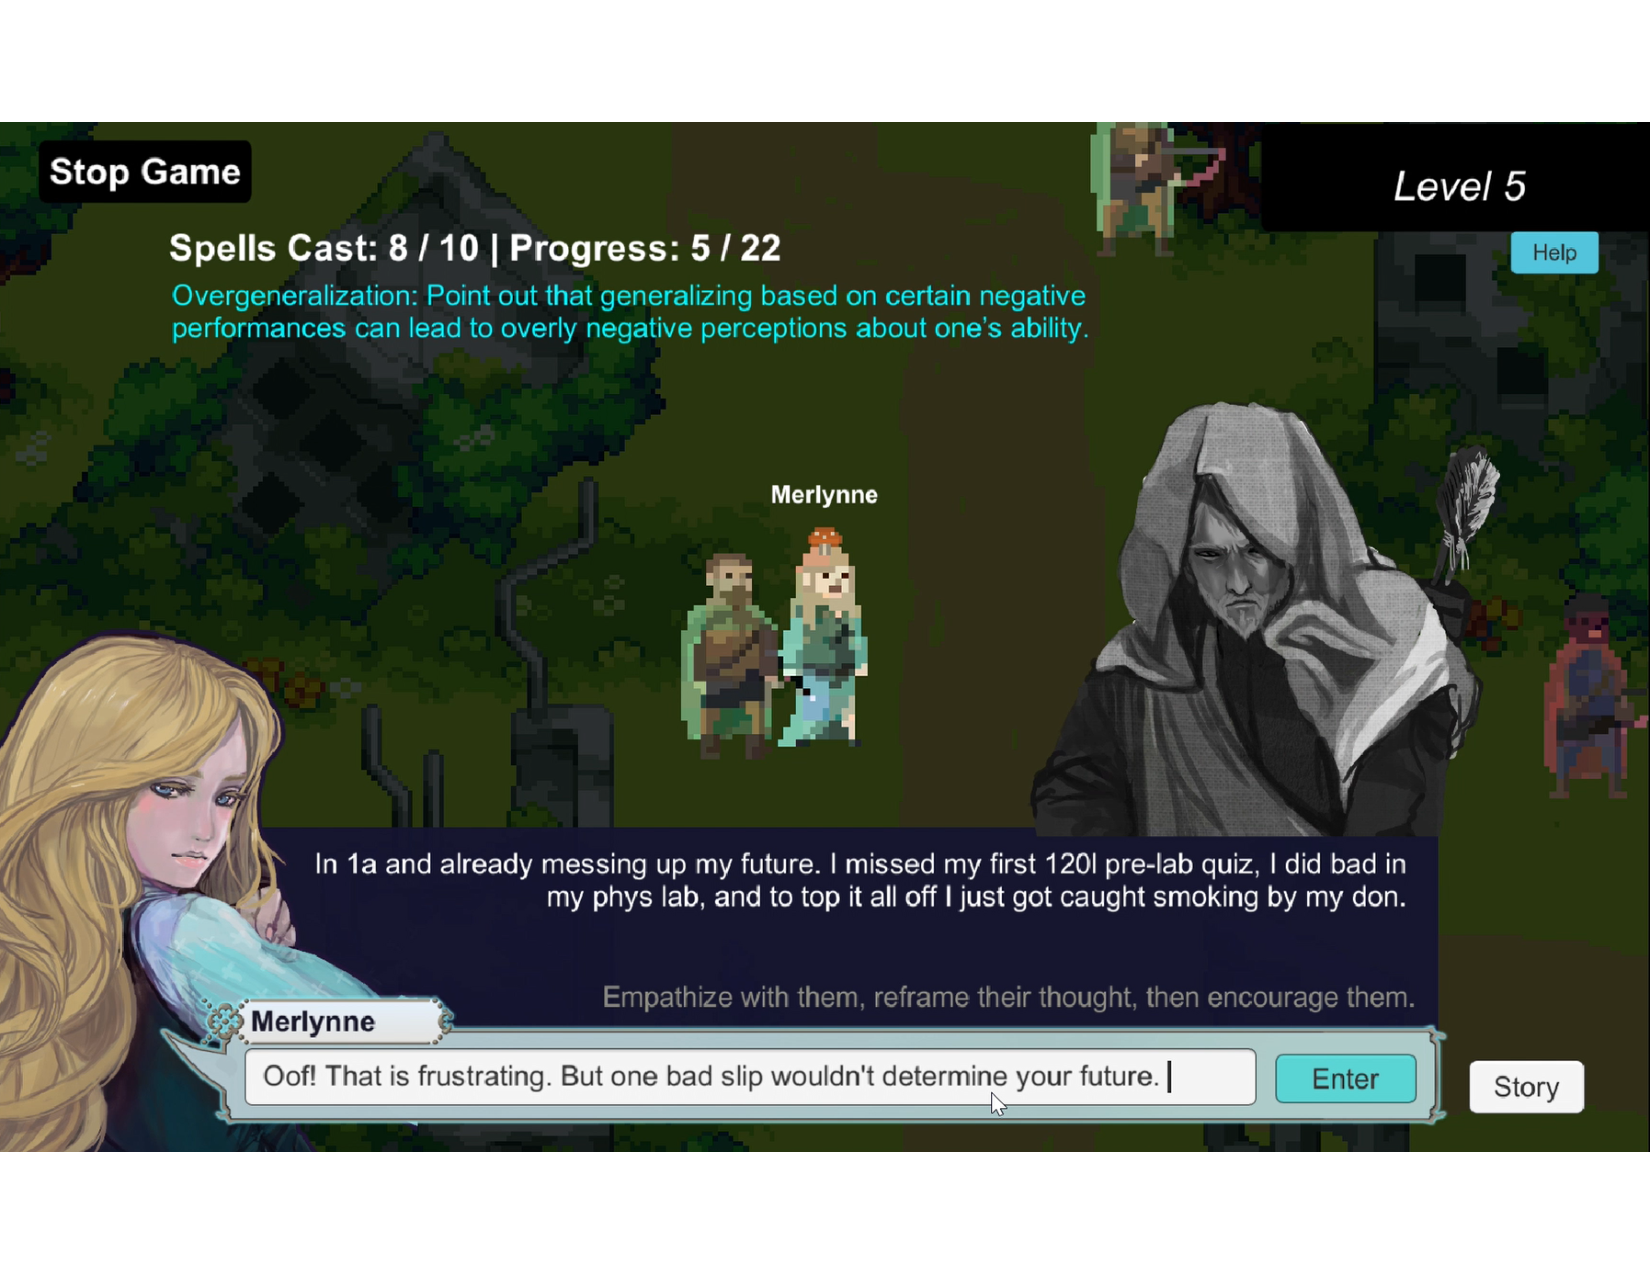
\includegraphics[width=.32\textwidth]{submission/figures/title1.pdf} 
%     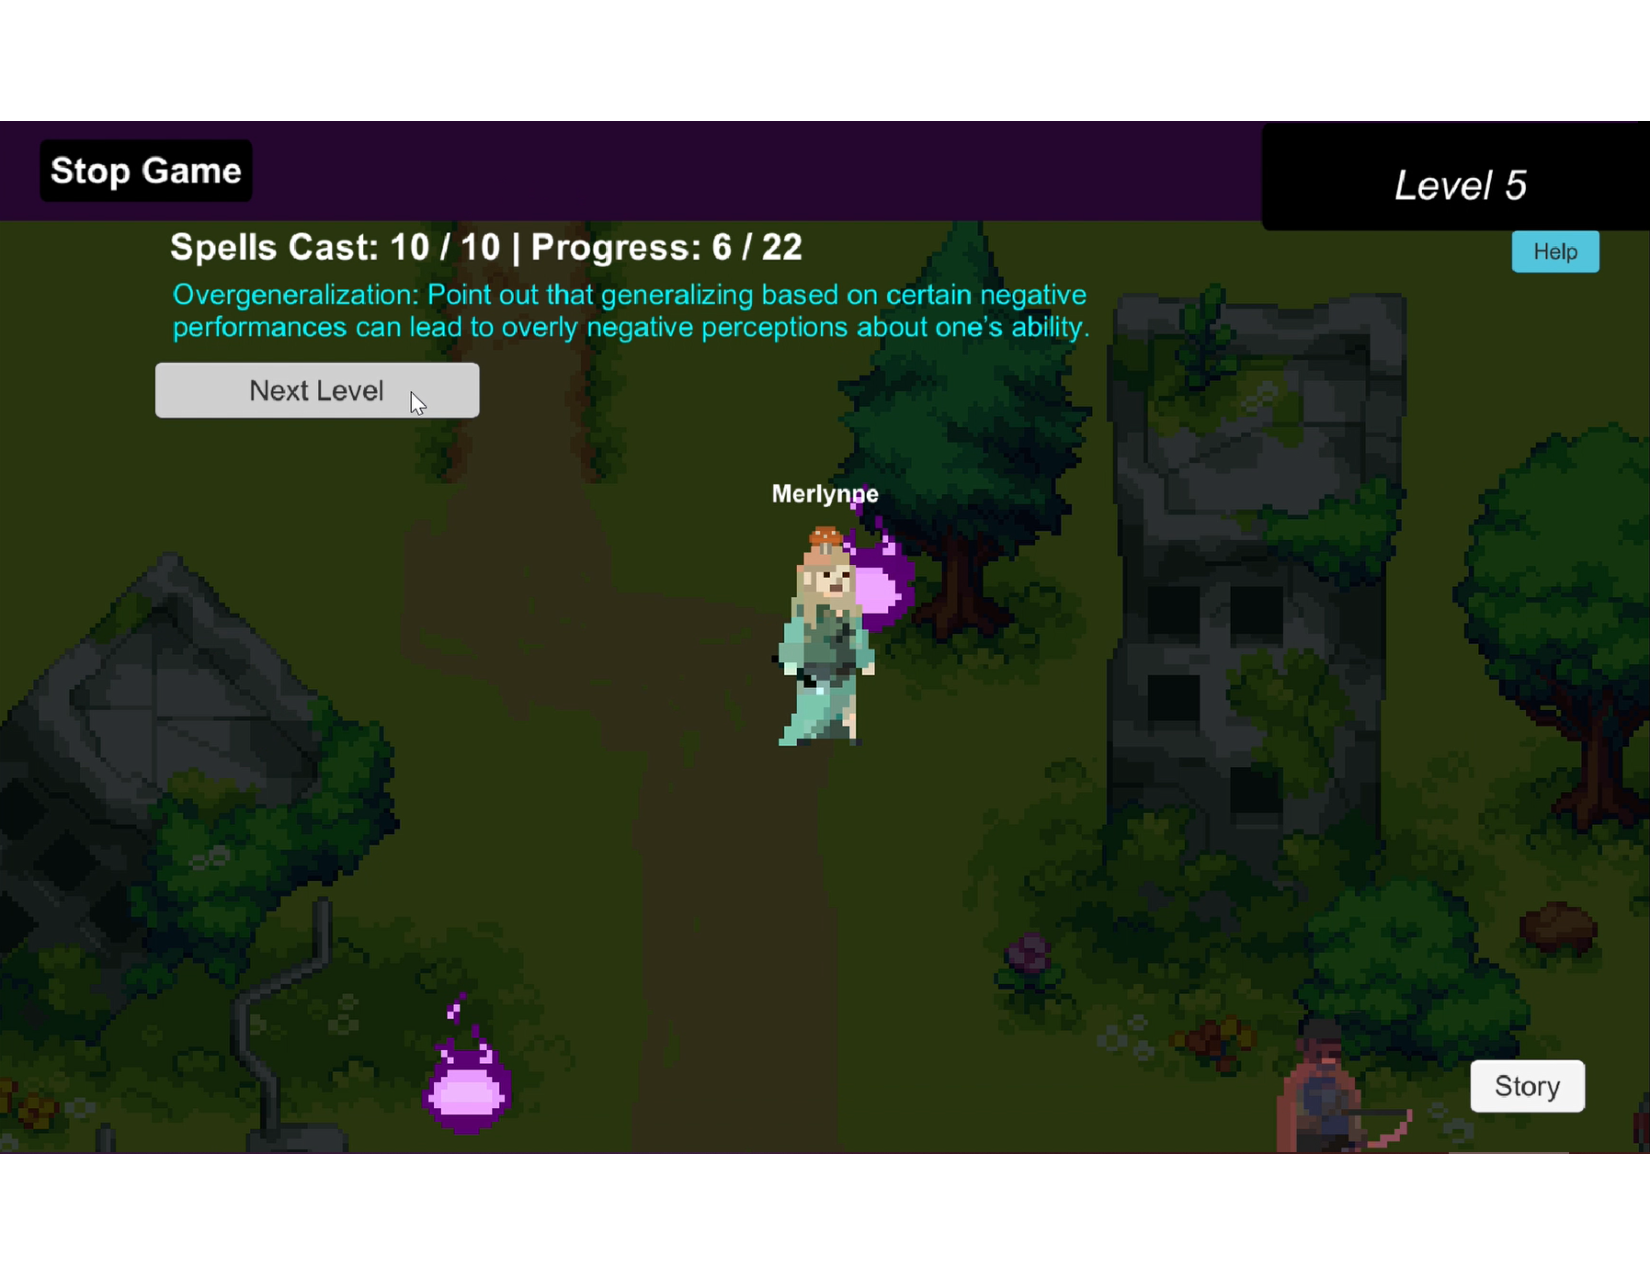
\includegraphics[width=.32\textwidth]{submission/figures/title2.pdf} 
%     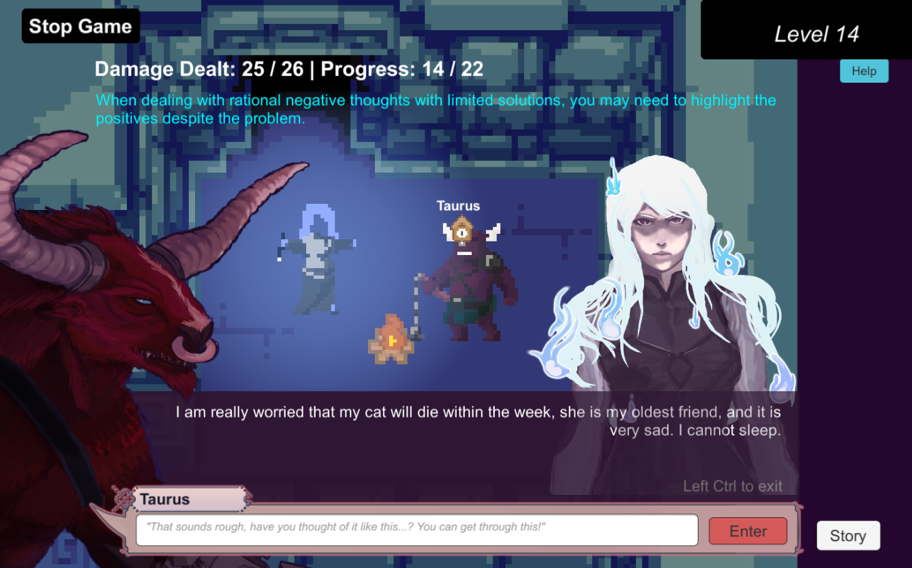
\includegraphics[width=.32\textwidth]{submission/figures/minotaur.pdf}
%     \caption{In \textit{Merlynne}, players unlock gameplay with CBT-based replies to negative Reddit posts in a fantasy role playing setting.}
%     \label{fig:teaser}
% }

\begin{document}
\title{\plaintitle}

\numberofauthors{3}
\author{%
  \alignauthor{Leave Authors Anonymous\\
    \affaddr{for Submission}\\
    \affaddr{City, Country}\\
    \email{e-mail address}}\\
  \alignauthor{Leave Authors Anonymous\\
    \affaddr{for Submission}\\
    \affaddr{City, Country}\\
    \email{e-mail address}}\\
  \alignauthor{Leave Authors Anonymous\\
    \affaddr{for Submission}\\
    \affaddr{City, Country}\\
    \email{e-mail address}}\\
}

\maketitle

\begin{abstract}
My new CHI paper
\end{abstract}

%
% The code below should be generated by the tool at
% http://dl.acm.org/ccs.cfm
% Please copy and paste the code instead of the example below.
%
\begin{CCSXML}
<ccs2012>
<concept>
<concept_id>10003120.10003130.10011762</concept_id>
<concept_desc>Human-centered computing~Empirical studies in collaborative and social computing</concept_desc>
<concept_significance>500</concept_significance>
</concept>
</ccs2012>
\end{CCSXML}

\ccsdesc[500]{Human-centered computing~Empirical studies in collaborative and social computing}

%\ccsdesc[500]{Computer systems organization~Embedded systems}
%\ccsdesc[300]{Computer systems organization~Redundancy}
%\ccsdesc{Computer systems organization~Robotics}
%\ccsdesc[100]{Networks~Network reliability}

% Author Keywords
\keywords{\plainkeywords}

% Print the classficiation codes
\printccsdesc


\vspace{2em}
\begin{quote}
    \emph{Great things are done by a series of small things brought together. --- Vincent Van Gough}
\end{quote}


%%%%%%%%%%%%%%%%%%%%%%%%%%%%%%%%%%%%%%%%%%%%%%%%%%%%%%%%%%%%%%%%%%%%%%%%%%%%%
\section{Introduction}
%%%%%%%%%%%%%%%%%%%%%%%%%%%%%%%%%%%%%%%%%%%%%%%%%%%%%%%%%%%%%%%%%%%%%%%%%%%%%

Even the most experienced researchers are constantly looking for ways to improve their papers. And there are many different aspects of a paper to improve on: from high-level concerns like experimental design, positioning the paper within the literature, and consideration of ethical issues, to sweating the details in a statistical analyis, or getting that graph \emph{just right} to show off your earth-shattering results. But sometimes it's hard to put all the pieces together. That's where this project comes in. 

This project --- CHI Zen, a play on the words `KaiZen' (\begin{CJK}{UTF8}{min}改善\end{CJK}) or `continuous improvement' --- describes common pitfalls and best practices based on my experience writing papers for a number of years. That experience reflects some of my own preferences, but also a lot that I've learned from working with other HCI researchers. It also contains a \emph{lot} of examples that you are free to copy, modify, or re-use as often as you'd like. The goal is to have something of an \emph{information zoo} \cite{heer2010tour} that can help you think about how to best visualize results, and hopefully make the process of creating that visualization easy, too. 

This document, also provides a sample reference for ``IDEA Plots,'' a set of templates that I developed for \texttt{PGFPlots}. Please use IDEA Plots if you find it useful. If you do, I'd love to hear about it, and if you have any ways to imrpove the templates. You might also prefer to use a different graphing package, and that's cool too. The examples contained in this document hopefully can provide tips or shortcuts for use in your own papers. I suspect that you can generate more or less the same graphs with your tool of choice. 

Finally, my intention in making this project available via GitHub is to allow it to grow. If you find it useful, please drop me a line. If you find a way to improve it, please push the changes to GitHub. It might also just be an important prompt to have a conversation about best practices, or an opportunity to explore different ways of thinking about or presenting research. In any case, I hope that it's an opportunity to think about how we can improve our research practices, one small step at a time. 




\vspace{2em}
\begin{center}
    \emph{Excellence is not a destination, it is a continuous journey that never ends.  --- Brian Tracy}
\end{center}

%%%%%%%%%%%%%%%%%%%%%%%%%%%%%%%%%%%%%%%%%%%%%%%%%%%%%%%%%%%%%%%%%%%%%%%%%%%%%
\section{\LaTeX\ and IDEA Plots}
%%%%%%%%%%%%%%%%%%%%%%%%%%%%%%%%%%%%%%%%%%%%%%%%%%%%%%%%%%%%%%%%%%%%%%%%%%%%%

\LaTeX is far from a perfect writing tool. For one thing, it's a `typesetting environment' and not a word processor, so little things like the difference between a ` and a ' can end up being important. When you're writing a paper, you generally want to focus on the words you're writing, and not getting the syntax right. So why use \LaTeX?

\begin{enumerate}
    \item Most formatting is done `for free' by the SIG CHI template, and it does a great job of this for you
    \item The University of Waterloo provides a Pro Overleaf account (think Google Docs for academic writing) if you login with your UW userid
    \item \LaTeX\ integrates well with other (free) tools like R, PGFPLots, etc. 
    \item Papers get rejected all the time, and reformatting is very fast and easy
\end{enumerate}

Since \LaTeX\ can be complex, this project also embodies some changes to the template that make our typical workflow a little easier:

\begin{enumerate}
    \item Sections are separated out into files, so that authors can edit each section without interrupting each other
    \item Additional packages:
    \item IDEA Plots --- see below. 
    \item ... 
\end{enumerate}



\subsection{PGFPlots and IDEA Plots}
As as I was completeing my PhD, I decided to spend some time trying to learn to make better figures since this was something I expected to spend a lot of time doing over the rest of my career, and I might as well think about how to do it well from the start. Some of the things I'd hoped to improve on were using scalable graphics, having better control over the width/height of figures, and being able to use experimental data itself to create the images (better fit with a typical academic workflow). I also prefer a minimalist feel, and wanted my papers to reflect that (And even if you prefer something different, this is a good starting point, you can always make things more complex where needed). 

So after doing some research, I found that \texttt{PGFPlots} was a good fit for my needs. But it wasn't perfect, and in particular can be complicated to get right. So in the interest of saving the time of re-inventing the wheel, and (hopefully) enabling others to use my work for their own papers, I decided to create a set of templates that would encapsulate the common types of graphs I use in HCI research. I called these templates \texttt{IDEA Plots}. As I developed the templates, they grew to include style choices, colour palettes, and some common shortcuts for layout. I expect they'll continue to evolve for a while to come.  

All of the examples in this document use the templates from \texttt{IDEA Plots}, with some in-place customization based on the needs of the graph. If you'd like to use those templates in your own work, be sure to include \texttt{IDEAPlots.tex} in your own project, and to \texttt{\textbackslash include\{IDEAPlots.tex\}} early on in your paper.  



%%%%%%%%%%%%%%%%%%%%%%%%%%%%%%%%%%%%%%%%%%%%%%%%%%%%%%%%%%%%%%%%%%%%%%%%%%%%%
%\section{GAME DESIGN}
%%%%%%%%%%%%%%%%%%%%%%%%%%%%%%%%%%%%%%%%%%%%%%%%%%%%%%%%%%%%%%%%%%%%%%%%%%%%%





\newpage
\vspace{2em}
\begin{center}
    \emph{If you define the problem correctly, you almost have the solution. --- Steve Jobs}
\end{center}

%%%%%%%%%%%%%%%%%%%%%%%%%%%%%%%%%%%%%%%%%%%%%%%%%%%%%%
\section{Tables}
%%%%%%%%%%%%%%%%%%%%%%%%%%%%%%%%%%%%%%%%%%%%%%%%%%%%%%
As a rule of thumb, if you can show your data with a table, consider doing that first. Tables are quite effective for showing real data, and usually easy to interpret. The Vis literature even says that tables might be more convincing for a skeptical audience \citep{pandey2014persuasive}!

In general, I suggest the following guidelines for formatting: 
\begin{enumerate}
    \item Remove vertical lines
    \item Only use horizontal lines where necessary
    \item Use \texttt{ \textbackslash toprule}, \texttt{ \textbackslash midrule}, and \texttt{ \textbackslash bottomrule} to frame your table
\end{enumerate}

You can see an example in \autoref{tab:exampletable}, below.

\begin{center}
\begin{table*}[htbp!]
\small
\begin{center}
\begin{tabular}{l l l l l}
\toprule
Condition & \multicolumn{4}{l}{Teamwork Measures}\\
\cmidrule(r){2-5}
& \multicolumn{2}{l}{Measure 1} & Measure 2 & Measure 3 \\
\cmidrule(r){2-3} 
&  Sub 1 & Sub 2 &  \\ 


\midrule


Condition 1 & .478 & .468 & 1.68 & 12.3  \\
                  & (.0259) & (.031) & (.703) & (5.93) \\
\\

Condition 2 & .444 & .451 & 1.32 & 18.4 \\
                              & (.0478) & (.0585) & (.319) & (2.76) \\
\\

Condition 3 &  & .410 &  2.857 &  \\
                     &        & (.0384)  & (.350) & \\
\\


ANOVA Results & $F_{(1,12)} = 2.27,$ & $F_{(2,18)} = 2.76,$  & $F_{(2,18)} = 16.16,$ & $F_{(1,12)} = 6.16,$ \\
                          & $p = .158$ & $p = .090  $ &  $p < .0001$* &  $p = 0.029$ * \\
\bottomrule
\end{tabular}

\caption[a]{Mean values and standard deviations (in parentheses) for teamwork measures, and ANOVA results for comparisons between experimental conditions. Significant results denoted by *.}
\label{tab:exampletable}
\end{center}
\end{table*}
\end{center}

%%%%%%%%%%%%%%%%%%%%%%%%%%%%%%%%%%%%%%%%%%%%%%%%%%%%%%%%%%%%%%%%%%%%%%%%%%%%%
\section{Showing Your Data}
%%%%%%%%%%%%%%%%%%%%%%%%%%%%%%%%%%%%%%%%%%%%%%%%%%%%%%%%%%%%%%%%%%%%%%%%%%%%%


- Figures and Tables in your results section often provide reviewers a first look at your results
- can also make the often dense results section more accessible to readers who are unfamiliar with your research area
- for readers with specific experience, particularly in replicated experimental settings such as a Fitts's Law study, can be the most important summary of research results in the paper 


Some rules of thumb from Munzer \cite{munznervisualization}:
\begin{enumerate}
	\item No unjustified 3D
	\item No unjustified 2D
	\item Eyes beat memory
	\item Get it right in Black and White
	\item Function first, form next
\end{enumerate}


Munzer \cite{munznervisualization}, and in particular Chapter 5, is a useful resource for determining which Marks and Channels to use in a graph, and lists them in order of effectiveness

- the style suggested in this document is informed and inspired by Tufte \cite{tufte1983visual}, who emphasizes minimalist presentation of quantitative data. Tufte's principles of information visualization 

 
 
%  For example, some good examples:
% Bartneck and Hu \cite{Bartneck:2009:SAC:1518701.1518810}


% Senellart \cite{Senellart:2013:DYR:2513166.2514938} discusses some useful cases of `bad' style, which superficially may appear to be picky but offer important guidance towards submitting polished papers. 
 
 
% Munzer \cite{Munzner:2008:PPW:1422919.1422927} 
% - some good advice in general, but more focused on info vis research

% - text is large and legible
% - all axes are labelled, including units of measure
% - axes start at 0, unless explicitly justified (for a good reason!)













%%%%%%%%%%%%%%%%%%%%%%%%%%%%%%%%%%%%%%%%%%%%%%%%%%%%%%%%%%
\subsection{Comparing Performance: Bar Charts and Box Plots}
%%%%%%%%%%%%%%%%%%%%%%%%%%%%%%%%%%%%%%%%%%%%%%%%%%%%%%%%%%

- common to compare performance, efficiency, error rate, or other dependent measures between two study groups. For example, our new technique for 3D pointing, compared to a computer mouse. 

- most simple way of doing so is to show the means and standard error in a bar graph, and this is commonly accepted throughout the ACM. 
- For example, Figure \ref{bargraph} is an example drawn from a UIST publication \cite{REF}.


\begin{figure}
\begin{tikzpicture}
\begin{axis}[IDEA bar,
        symbolic x coords={non-occluded,occluded},
        xtick = {non-occluded,occluded},
        enlarge x limits=0.5,
	    ymin = 0, ymax = 10,
        ylabel = {Selection Time (s)},
        width=\columnwidth,
        height = 5cm,
]

%Depth Ray
\addplot[style={draw=none,fill=AHSLight},error bars/.cd, y dir = both, y explicit, error bar style={black}]
coordinates {(occluded, 6.8)  +- (1.7,1.7)};
\addlegendentry{Depth Cursor}

%Tiltcasting
\addplot+[style={draw=none, fill=SchoolRedLight,line width = 0pt},error bars/.cd, y dir = both, y explicit, error bar style={black}]
coordinates {(non-occluded,3.24) +- (.712,.712)
		    (occluded,4)  +- (.922,.922)};
\addlegendentry{Tiltcasting}

%Smartcasting
\addplot+[style={draw=none, fill=EnvironmentLight},error bars/.cd, y dir = both, y explicit, error bar style={black}]
coordinates {(non-occluded, 2.10)  +- (.42,.42)};
\addlegendentry{Smartcasting}

\end{axis}
\end{tikzpicture}
\caption{An example bar graph with error bars. Data is specified in the latex file.}
\label{bargraph}
\end{figure}


- to be more accurate and descriptive, box plots are often used
- similar to a bar graph with error bars, but also indicate quartiles and outliers 
- typically, better practice to include a box plot when possible -- but can be substantially more difficult to create in Microsoft Word. 




%%%%%%%%%%%%%%%%%%%%%%%%%%%%%%%%%%%%%%%%%%%%%%%%%%%%%%%%%%
\subsection{Questionnaire Responses}
%%%%%%%%%%%%%%%%%%%%%%%%%%%%%%%%%%%%%%%%%%%%%%%%%%%%%%%%%%

- Common to want to show questionnaire respones, particularly to, e.g., Likert scale questions
- Jim's preference: stacked divergent bar graph

\begin{figure}
\begin{tikzpicture}
\pgfplotstableread[col sep = comma]{submission/data/Cleric_AvatarIdentificationStacked.csv}\ClericIdentificationData
\pgfplotstableread[col sep = comma]{submission/data/Monster_AvatarIdentificationStacked.csv}\MonsterIdentificationData

\begin{axis}[
    IDEA Likert,
    height = 6.5cm,
    width = .75\columnwidth,
    % Y AXIS
    symbolic y coords = {Ava_Conn,	Ava_WE,	AvavsPhys,	AvaVsPers,	AvaVsPhysIdeal,	AvaVsPersIdeal},
    ytick={Ava_Conn, Ava_WE, AvavsPhys, AvaVsPers, AvaVsPhysIdeal, AvaVsPersIdeal},
    yticklabels={Connectedness, Refer to \\ Avatar as ``We'', Physical \\ Similarity, Personality\\ Similarity, Physical Ideal, Ideal Personality},
    yticklabel style={align=right,font={\sffamily\small}},
    y axis line style={draw=none},
    y dir = reverse,
    ymajorgrids = false,
    % X AXIS
    xmin=-100, xmax=100,
    xlabel={\% of Responses},
    xlabel style = {font=\small\sffamily},
    xticklabel style = {font=\small\sffamily},
    xtick = {-100,-50,0,50,100},
    xticklabels = {100, 50, 0, 50, 100},
    extra x ticks = {-75, 75},
    extra x tick labels = {$\leftarrow$ Disagree, Agree $\rightarrow$},
    every extra x tick/.style={major tick length=0,yshift={-8pt}},
    ]
    \addplot[draw=none,fill=none, forget plot] coordinates {(0,Ava_Conn)(0,Ava_WE)(0,AvavsPhys)(0,AvaVsPers)(0,AvaVsPhysIdeal)(0,AvaVsPersIdeal)};
    \addplot[draw=none,fill=Cleric_3, forget plot, bar shift=.1cm] table [x expr={\thisrow{4}*-0.5},y=Measure] {\ClericIdentificationData};
    \addplot[draw=none,fill=Cleric_2, forget plot, bar shift=.1cm] table [x expr={\thisrow{3}*-1},y=Measure] {\ClericIdentificationData};
    \addplot[draw=none,fill=Cleric_1, forget plot, bar shift=.1cm] table [x expr={\thisrow{2}*-1}, y=Measure ] {\ClericIdentificationData};
    \addplot[draw=none,fill=Cleric_0, forget plot, bar shift=.1cm] table [x expr={\thisrow{1}*-1}, y=Measure ] {\ClericIdentificationData};
    \resetstackedplots
    \addplot[draw=none,fill=none, forget plot] coordinates {(0,Ava_Conn)(0,Ava_WE)(0,AvavsPhys)(0,AvaVsPers)(0,AvaVsPhysIdeal)(0,AvaVsPersIdeal)};
    \addplot[draw=none,fill=Monster_3, forget plot, bar shift=-.1cm] table [x expr={\thisrow{4}*-0.5},y=Measure] {\MonsterIdentificationData};
    \addplot[draw=none,fill=Monster_2, forget plot, bar shift=-.1cm] table [x expr={\thisrow{3}*-1},y=Measure] {\MonsterIdentificationData};
    \addplot[draw=none,fill=Monster_1, forget plot, bar shift=-.1cm] table [x expr={\thisrow{2}*-1}, y=Measure ] {\MonsterIdentificationData};
    \addplot[draw=none,fill=Monster_0, forget plot, bar shift=-.1cm] table [x expr={\thisrow{1}*-1}, y=Measure ] {\MonsterIdentificationData};
\end{axis}

\begin{axis}[
    IDEA Likert,
    height = 6.5cm,
    width = .75\columnwidth,
    % Y AXIS
    symbolic y coords = {Ava_Conn,	Ava_WE,	AvavsPhys,	AvaVsPers,	AvaVsPhysIdeal,	AvaVsPersIdeal},
    ytick={Ava_Conn, Ava_WE, AvavsPhys, AvaVsPers, AvaVsPhysIdeal, AvaVsPersIdeal},
    yticklabels={Connectedness, Refer to \\ Avatar as ``We'', Physical \\ Similarity, Personality\\ Similarity, Physical Ideal, Ideal Personality},
    yticklabel style={align=right,font={\sffamily\small}},
    y axis line style={draw=none},
    y dir = reverse,
    ymajorgrids = false,
    % X AXIS
    xmin=-100, xmax=100,
    xlabel={\% of Responses},
    xlabel style = {font=\small\sffamily},
    xticklabel style = {font=\small\sffamily},
    xtick = {-100,-50,0,50,100},
    xticklabels = {100, 50, 0, 50, 100},
    extra x ticks = {-75, 75},
    extra x tick labels = {$\leftarrow$ Disagree, Agree $\rightarrow$ },
    every extra x tick/.style={major tick length=0,yshift={-8pt}},
    ]
    \addplot[draw=none,fill=none, forget plot] coordinates {(0,Ava_Conn)(0,Ava_WE)(0,AvavsPhys)(0,AvaVsPers)(0,AvaVsPhysIdeal)(0,AvaVsPersIdeal)};
    
    \addplot[draw=none,fill=Cleric_3, forget plot, bar shift=.1cm] table [x expr={\thisrow{4}*0.5}, y=Measure ] {\ClericIdentificationData};
    \addplot[draw=none,fill=Cleric_4, forget plot, bar shift=.1cm] table [x expr={\thisrow{5}}, y=Measure ] {\ClericIdentificationData};
    \addplot[draw=none,fill=Cleric_5, forget plot, bar shift=.1cm] table [x expr={\thisrow{6}}, y=Measure ] {\ClericIdentificationData};
    \addplot[draw=none,fill=Cleric_6, forget plot, bar shift=.1cm] table [x expr={\thisrow{7}}, y=Measure ] {\ClericIdentificationData}; \label{plot:cleric6}
    \resetstackedplots
    \addplot[draw=none,fill=none, forget plot] coordinates {(0,Ava_Conn)(0,Ava_WE)(0,AvavsPhys)(0,AvaVsPers)(0,AvaVsPhysIdeal)(0,AvaVsPersIdeal)};
    \addplot[draw=none,fill=Monster_3, forget plot, bar shift=-.1cm] table [x expr={\thisrow{4}*0.5}, y=Measure ] {\MonsterIdentificationData};
    \addplot[draw=none,fill=Monster_4, forget plot, bar shift=-.1cm] table [x expr={\thisrow{5}}, y=Measure ] {\MonsterIdentificationData};
    \addplot[draw=none,fill=Monster_5, forget plot, bar shift=-.1cm] table [x expr={\thisrow{6}}, y=Measure ] {\MonsterIdentificationData};
    \addplot[draw=none,fill=Monster_6, forget plot, bar shift=-.1cm] table [x expr={\thisrow{7}}, y=Measure ] {\MonsterIdentificationData};
    %\addlegendimage{only marks, mark=o}
    %\addlegendimage{only marks, mark=o}
    %\legend{Neutral, Agree, Strongly Agree, Disagree,Strongly Disagree}
    after end axis/.code={
        \node at (axis cs:80,Ava_Conn) [anchor=east, ,font=\tiny] {\AsteriskBold};
        \node at (axis cs:80,Ava_WE) [anchor=east, font=\tiny] {\AsteriskBold};
        %\draw [white] (axis cs:0,AvaVsPersIdeal) -- (axis cs:0,Ava_Conn);
        %\draw [white] (axis cs:-50,AvaVsPersIdeal) -- (axis cs:-50,Ava_Conn);
        %\draw [white] (axis cs:50,AvaVsPersIdeal) -- (axis cs:50,Ava_Conn);
    }
    \coordinate (legend) at (axis description cs:1.15,.85);
\end{axis}

% this is a dummy `axis' environment only to create the legend
\matrix [
    matrix of nodes, 
    every node/.style={anchor=center}, 
    ] at (legend) {
        |[fill=Cleric_0]| & |[fill=Cleric_1]| & |[fill=Cleric_2]| & |[fill=Cleric_3]| & |[fill=Cleric_4]| & |[fill=Cleric_5]| & |[fill=Cleric_6]| & |[font=\small\sffamily]|Cleric \\
        |[fill=Monster_0]| & |[fill=Monster_1]| & |[fill=Monster_2]| & |[fill=Monster_3]| & |[fill=Monster_4]| & |[fill=Monster_5]| & |[fill=Monster_6]| & |[font=\small\sffamily]|Monster \\
    };
\end{tikzpicture}
    
\caption{Summary of avatar identification responses, based on 7-point Likert scales. Mann Whitney U tests revealed significant differences between \textsc{Avatar} groups for `Connectness' and `Refer to Avatar as We'. }
\label{fig:avatar_identification}
\end{figure}




%%%%%%%%%%%%%%%%%%%%%%%%%%%%%%%%%%%%%%%%%%%%%%%%%%%%%%%%%%
\subsubsection{Showing Trends over Time}
%%%%%%%%%%%%%%%%%%%%%%%%%%%%%%%%%%%%%%%%%%%%%%%%%%%%%%%%%%



\begin{figure}[t!]
\begin{tikzpicture}[baseline]
\begin{axis}[IDEA line,
	% Graph Options
	width=.475*\columnwidth,
	height=4cm,
	title=\texttt{r/stop\-drinking},
	% X Axis Options
	%date coordinates in=x,
	%date ZERO=2014-01-01,
    %xticklabel=\year,
    %xmin=2014-01-01,
    %xmax=2018-01-01,
    xlabel=Year,
	xtick={1,13,25,37,49},                              %% Jim: apologies... this is a hack
    xticklabels={2014,2015,2016,2017,2018},             %%      will figure out what's going on here if we have time later
	%xtick ={1,2,3,4,5,6,7,8,9},
	% Y Axis Options
	ylabel = Distinct Users / Active Threads,
	ylabel style = {font=\tiny},
	ymin = 0, ymax = 6000,
	ytick = {0,2000,4000,6000},
	ytick style = {font=\tiny},
    %legend image code/.code={\draw[#1] circle (0.1cm);}
]

\pgfplotstableread[col sep = comma]{submission/data/stopdrinking-usagebymonth.csv}\mydata;
\addplot+[draw=ScienceDark,fill=none,thick] table[x=index,y=users] {\mydata};
\addplot+[draw=ArtsLight,fill=none,thick] table[x=index,y=threads] {\mydata};

\end{axis}
\end{tikzpicture}%
%
\begin{tikzpicture}[baseline]
\begin{axis}[IDEA line,
	% Graph Options
	width=.475*\columnwidth,	
	height=4cm,
	title=\texttt{r/Opiates\-Recovery},
	% X Axis Options
	xtick={1,13,25,37,49},                              %% Jim: apologies... this is a hack
    xticklabels={2014,2015,2016,2017,2018},             %%      will figure out what's going on here if we have time later
	%date coordinates in=x,
	%date ZERO=2014-01-01,
    %xticklabel=\year,
    %xmin=2014-01-01,
    %xmax=2018-01-01,
	xlabel = Year,
	%xtick ={1,2,3,4,5,6,7,8,9},
	% Y Axis Options
	ylabel = Distinct Users / Active Threads,
	ylabel style = {font=\tiny},
	ymin = 0, ymax = 800,
	ytick = {0,200,400,600,800},
	ytick style = {font=\tiny},
	legend style={at={(0.5,-1)},anchor=south}
    %legend image code/.code={\draw[#1] circle (0.1cm);}
]

\pgfplotstableread[col sep = comma]{submission/data/opiaterecovery-usagebymonth.csv}\mydata;
\addplot+[draw=ScienceDark,fill=none,thick] table[x=index,y=users] {\mydata};
\addlegendentry{Distinct Users}
\addplot+[draw=ArtsLight,fill=none,thick] table[x=index,y=threads] {\mydata};
\addlegendentry{Active Threads}

\end{axis}
\end{tikzpicture}
%\setlength{\belowcaptionskip}{-20pt}
\caption{Distinct users and active threads for \texttt{r/stop\-drinking} (top) and \texttt{r/Opiates\-Recovery} (bottom) showing that both counts are experiencing an upwards trend over time for both subreddits.} 

\label{fig:activity}
\end{figure}



\begin{figure*}[tb!]
\begin{center}
\begin{tikzpicture}
\begin{groupplot}[
   group style={
       group size=1 by 5,
       x descriptions at=edge bottom,
       y descriptions at=edge left,
       vertical sep=1pt,
       horizontal sep=0pt},
  IDEA tufte panel, 
	% X Axis
	width=\columnwidth,
	xmin = 1990, xmax = 2015,
	xtick = {1990,1994,1998,2002,2006,2010,2015},
	x tick label style={font=\small,rotate=90, /pgf/number format/1000 sep=},
	axis line style={thick},
	% Y Axis
	ytick={10,20,30,40,50,60,70,80,90},
        ymin = 0,
        ymax = 50,
      ]


% Bibliographic
\nextgroupplot[bar width=7pt, height = 2.25cm, ymax = 25, title={Bibliographic}]
\addplot+[draw=none, fill=black!50] 
 coordinates {(1990,20) (1992,4) (1994,0) (1996,0) (1998,2) (2000,0) (2002,0) (2004,2) (2006,2) (2008,1) (2010,0) (2011,0) (2012,0) (2013,1) (2014,0) (2015,1) };       
  
% Not Empirical      
\nextgroupplot[bar width=7pt, height = 3.5cm, ymax=70, title={Not Empirical}]
\addplot+[draw=none, fill=black!50] 
coordinates {(1990,37) (1992,55) (1994,33) (1996,38) (1998,54) (2000,35) (2002,20) (2004,18) (2006,24) (2008,13) (2010,5) (2011,31) (2012,9) (2013,4) (2014,6) (2015,7) };

% Explanatory
\nextgroupplot[bar width=7pt, height = 3cm, title={Explanatory}]
\addplot+[draw=none, fill=black!50]  
coordinates {(1990,3) (1992,4) (1994,5) (1996,0) (1998,0) (2000,5) (2002,15) (2004,16) (2006,29) (2008,25) (2010,21) (2011,16) (2012,8) (2013,14) (2014,15) (2015,12) };

% D & E
\nextgroupplot[bar width=7pt, ymax=60, height = 3.5cm, title={Design and Evaluation}]
\addplot+[draw=none, fill=blue!50] 
coordinates {(1990,17) (1992,13) (1994,26) (1996,22) (1998,15) (2000,27) (2002,39) (2004,35) (2006,23) (2008,19) (2010,21) (2011,10) (2012,28) (2013,26) (2014,24) (2015,22) };

% Descriptive
\nextgroupplot[bar width=7pt, ymax = 70, height = 3.5cm, title={Descriptive}]
\addplot+[draw=none,fill=black!50]
coordinates {(1990,23) (1992,23) (1994,36) (1996, 40) (1998,29) (2000,32) (2002,27) (2004,29) (2006,23) (2008,42) (2010,53) (2011,42) (2012,55) (2013,55) (2014,55) (2015,58) };


\end{groupplot}
\end{tikzpicture}
\caption{An example of Tufte's stacked panel graph, which presents the same information as a stacked bar graph but better enables comparisons across each vertical dimension. Best practice is to use black and white when possible, with sparing colour for emphasis where appropriate. }
\label{stackedpanel}
\end{center}
\end{figure*}




\begin{figure}
\begin{tikzpicture}
\begin{groupplot}[
   group style={
       group size=1 by 5,
       x descriptions at=edge bottom,
       y descriptions at=edge left,
       vertical sep=10pt,
       horizontal sep=0pt},
  IDEA line,
	% Graph Options
	height=3cm,
	 separate axis lines,
	% X Axis Options
	xmin=0, xmax= 35,
	xtick={1,5,10,15,20,25,30, 35},
	%date coordinates in=x,
	%date ZERO=2014-01-01,
    %xticklabel=\year,
    %xmin=2014-01-01,
    %xmax=2018-01-01,
	xlabel = Number of NPC Requests,
	xlabel style = {font=\small\sffamily},
    xticklabel style = {font=\small\sffamily},
	%xtick ={1,2,3,4,5,6,7,8,9},
	% Y Axis Options
	%ylabel = Proportion of Responses,
	ymajorgrids = false,
	ylabel shift = -.3cm,
	ymin = 0, ymax = 1,
	ytick = {0, 1.00},
	ylabel style = {font=\small\sffamily},
    yticklabel style = {font=\small\sffamily},
	%ytick style = {font=\tiny},
	title style = {yshift=-.75cm,font=\sffamily\small}
]
\pgfplotstableread[col sep = comma]{submission/data/CBT_PropOverTime.csv}\cbtovertimedata;

\nextgroupplot[xtick style = {white}, title style = {yshift=+.35cm,font=\sffamily\small}, title={Not Damaging}]
\addplot+[mark=*, mark size=1.5pt, draw=gray, only marks,fill=gray,thin] table[x=Query,y=NotDamaging] {\cbtovertimedata};
\addplot [solid, draw=black, fill=none,ultra thick] table[y={create col/linear regression={y=NotDamaging}}] {\cbtovertimedata};
%\addlegendentry{Not Damaging}

\nextgroupplot[xtick style = {white}, title={Empathize}]
\addplot+[mark=*, mark size=1.5pt, draw=gray, only marks,fill=gray,thin] table[x=Query,y=Empathize] {\cbtovertimedata};
\addplot [solid, draw=black, fill=none,ultra thick] table[y={create col/linear regression={y=Empathize}}] {\cbtovertimedata};
%\addlegendentry{Empathize}

\nextgroupplot[xtick style = {white}, title style = {yshift=+.25cm,font=\sffamily\small}, title={Reframe}]
\addplot+[mark=*, mark size=1.5pt, draw=gray, only marks,fill=gray,thin] table[x=Query,y=Reframe] {\cbtovertimedata};
\addplot [solid, draw=black, fill=none,ultra thick] table[y={create col/linear regression={y=Reframe}}] {\cbtovertimedata};
%\addlegendentry{Reframe}

\nextgroupplot[xtick style = {white}, title={Encourage}]
\addplot+[mark=*, mark size=1.5pt, draw=gray, only marks,fill=gray,thin] table[x=Query,y=Encourage] {\cbtovertimedata};
\addplot [solid, draw=black, fill=none,ultra thick] table[y={create col/linear regression={y=Encourage}}] {\cbtovertimedata};
%\addlegendentry{Encourage}

\nextgroupplot[title={Solution}]
\addplot+[mark=*, mark size=1.5pt, draw=gray, only marks,fill=gray,thin] table[x=Query,y=Solution] {\cbtovertimedata};
\addplot [solid, draw=black, fill=none,ultra thick] table[y={create col/linear regression={y=Solution}}] {\cbtovertimedata};
%\addlegendentry{Solution}


%\addplot+[mark=x, only marks,draw=Monster_0,fill=none,semithick] table[x=Query,y=Proportion, y error plus=CI-upper, y error minus=CI-lower] {\barbariansolutiondata};
%\addlegendentry{Monster}
%\addplot [draw=Monster_0, fill=none,ultra thick] table[y={create col/linear regression={y=Proportion}}] {\barbariansolutiondata};

\end{groupplot}
\end{tikzpicture}

%\setlength{\belowcaptionskip}{-20pt}
\caption{The proportion of responses that were classified as meeting five criteria: Empathize, Reframe, Encourage, Solution, and Not Damaging. The three categories related to CBT, Empathize, Reframe, and Encourage, were found to decrease over time ($p=0.05$). However, we did not find these changes for Solution and Not Damaging. 
%decreased over time for all participants, however responses by participants in the \textsc{Cleric} group decreased more quickly than those in the \textsc{Monster} group.
} 

\label{fig:SolutionsOverQueryNumber}
\end{figure}
























%%%%%%%%%%%%%%%%%%%%%%%%%%%%%%%%%%%%%%%%%%%%%%%%%%%%%%%%%%%%%%%%%%%%%%%%%%%%%
%\section{Discussion \& Implications}
%%%%%%%%%%%%%%%%%%%%%%%%%%%%%%%%%%%%%%%%%%%%%%%%%%%%%%%%%%%%%%%%%%%%%%%%%%%%%


%%%%%%%%%%%%%%%%%%%%%%%%%%%%%%%%%%%%%%%%%%%%%%%%%%%%%%%%%%%%%%%%%%%%%%%%%%%%%
%\section{Limitations}
%%%%%%%%%%%%%%%%%%%%%%%%%%%%%%%%%%%%%%%%%%%%%%%%%%%%%%%%%%%%%%%%%%%%%%%%%%%%%



%%%%%%%%%%%%%%%%%%%%%%%%%%%%%%%%%%%%%%%%%%%%%%%%%%%%%%%%%%%%%%%%%%%%%%%%%%%%%
%\section{Conclusions}
%%%%%%%%%%%%%%%%%%%%%%%%%%%%%%%%%%%%%%%%%%%%%%%%%%%%%%%%%%%%%%%%%%%%%%%%%%%%%



%%%%%%%%%%%%%%%%%%%%%%%%%%%%%%%%%%%%%%%%%%%%%%%%%%%%%%%%%%%%%%%%%%%%%%%%%%%%%
\section{Acknowledgements}
%%%%%%%%%%%%%%%%%%%%%%%%%%%%%%%%%%%%%%%%%%%%%%%%%%%%%%%%%%%%%%%%%%%%%%%%%%%%%


\newpage
%\bibliographystyle{SIGCHI-Reference-Format}
\bibliographystyle{ACM-Reference-Format}
\bibliography{submission/bibliography.bib}

%\input{submission/11-appendix.tex}

\end{document}